%; whizzy paragraph
%; whizzy-paragraph "^\\\\dancersection"
% -initex iniptex -latex platex -format platex -bibtex jbibtex -fmt fmt
% 以上 whizzytex を使用する場合の設定。

%     Tokyo Debian Meeting resources
%     Kansai Debian Meeting resources
%     Copyright (C) 2012 Junichi Uekawa
%     Copyright (C) 2012 Nobuhiro Iwamatsu
%     Copyright (C) 2012 Koichi Akabe

%     This program is free software; you can redistribute it and/or modify
%     it under the terms of the GNU General Public License as published by
%     the Free Software Foundation; either version 2 of the License, or
%     (at your option) any later version.

%     This program is distributed in the hope that it will be useful,
%     but WITHOUT ANY WARRANTY; without even the implied warranty of
%     MERCHANTABILITY or FITNESS FOR A PARTICULAR PURPOSE.  See the
%     GNU General Public License for more details.

%     You should have received a copy of the GNU General Public License
%     along with this program; if not, write to the Free Software
%     Foundation, Inc., 51 Franklin St, Fifth Floor, Boston, MA  02110-1301 USA

%  preview (shell-command (concat "evince " (replace-regexp-in-string "tex$" "pdf"(buffer-file-name)) "&"))
% 画像ファイルを処理するためにはebbを利用してboundingboxを作成。
%(shell-command "cd image2012-natsu; ebb *.png")

% progress memo:
% 2015/12-2016/05がマージ対象
% イベント等でない場合は理由を書くこと。
% 必要な変更点は FIXME で記録しています。

%%ここからヘッダ開始。

\documentclass[mingoth,a4paper]{jsarticle}
\usepackage{monthlyreport}
\usepackage{supertabular}
\usepackage{subfigure}
\renewcommand*\thesubfigure{}

\usepackage{comment}

% ルビ for 201312tokyo
\def\ruby#1#2{%
\leavevmode
\setbox0=\hbox{#1}\setbox1=\hbox{\tiny#2}%
\ifdim\wd0>\wd1 \dimen0=\wd0 \else \dimen0=\wd1 \fi
\hbox{\kanjiskip=\fill
\vbox{\hbox to \dimen0{\tiny \hfil#2\hfil}%
\nointerlineskip
\hbox to \dimen0{\hfil#1\hfil}}}}

% section の代わりの環境 -- 改訂する。
\renewcommand{\dancersection}[2]{%
\newpage
あんどきゅめんてっど でびあん 2016年夏号
%
% top line
\vspace{0.1mm}\\
{\color{dancerdarkblue}\rule{\hsize}{2mm}}

%
% middle text
%
\begin{minipage}[t]{0.6\hsize}
\color{dancerdarkblue}
\vspace{1cm}
\section{#1}
\hfill{}#2\\
\end{minipage}
\begin{minipage}[t]{0.4\hsize}
\vspace{-2cm}
\hfill{}
\includegraphics[height=8cm]{image200502/openlogo-nd.eps}\\
\vspace{-5cm}
\end{minipage}
%
% bottom line
{\color{dancerlightblue}\rule{0.66\hsize}{2mm}}
%
\vspace{2cm}
}
% end of dancersection.

\begin{document}

\begin{titlepage}
\thispagestyle{empty}

\hspace*{-2.5cm}

\includegraphics{image2012-natsu/gudeb.eps}\\
\vspace*{0.1cm}

\vspace*{2cm}
\rotatebox{10}{\fontsize{32}{32} {\gt 東京エリア/関西Debian勉強会}}

\vspace*{-1.5cm}
\hspace*{11cm}
\includegraphics[height=6cm]{image200502/openlogo-nd.eps}\\
\vspace*{0.1cm}
\hfill あんどきゅめんてっど でびあん 2016年夏号 2016年8月14日 初版発行
\end{titlepage}

\newpage
\thispagestyle{empty}\mbox{}
\newpage

\setcounter{page}{1}
\begin{minipage}[]{0.2\hsize}
 \definecolor{titleback}{gray}{0.9}
 \colorbox{dancerlightblue}{\rotatebox{90}{\fontsize{80}{80}
{\gt \color{dancerdarkblue}デビアン勉強会} }}
\end{minipage}
\begin{minipage}[]{0.8\hsize}
\hrule
\vspace{1mm}
\hrule
\setcounter{tocdepth}{1}
{\small
\begin{multicols}{2}
  \tableofcontents
\end{multicols}
} %FIXME: does not fit in one column! しかし二段にするとあまり美しくない? 真ん中のあたりで章番号とページ数の番号が近くにあるのがバランス良くない気がする
\vspace{1mm}
\hrule
\vspace{3cm}

\end{minipage}

% FIXME: 本文を追加すること。
%-------------------------------------------------------------------------------
\dancersection{Introduction}{野島 貴英,かわだ てつたろう}
%-------------------------------------------------------------------------------

\subsection{東京エリアDebian勉強会}

 Debian勉強会へようこそ。これからDebianの世界にあしを踏み入れると
 いう方も、すでにどっぷりとつかっているという方も、月に一回Debianについ
 て語りませんか?

 Debian勉強会の目的は下記です。

\begin{itemize}
 \item \underline{Debian Developer} (開発者)の育成。
 \item 日本語での「\underline{開発に関する情報}」を整理してまとめ、アップデートする。
 \item \underline{場}の提供。
 \begin{itemize}
  \item 普段ばらばらな場所にいる人々が face-to-face で出会える場を提供
	する。
  \item Debian のためになることを語る場を提供する。
  \item Debianについて語る場を提供する。
 \end{itemize}
\end{itemize}

 Debianの勉強会ということで究極的には参加者全員がDebian Packageをがりがり
 と作るスーパーハッカーになった姿を妄想しています。情報の共有・活用を通し
 て Debianの今後の能動的な展開への土台として、「場」としての空間を提供す
 るのが目的です。

\subsection{関西 Debian 勉強会}

 関西 Debian 勉強会はDebian GNU/Linux のさまざ
 まなトピック(新しいパッケージ、Debian 特有の機能の仕組、Debian 界隈で起
 こった出来事、などなど)について話し合う会です。

 目的として次の三つを考えています。
 \begin{itemize}
  \item メーリングリストや掲示板ではなく、直接顔を合わせる事での情報交換の促進
  \item 定期的に集まれる場所
  \item 資料の作成
 \end{itemize}

 それでは、楽しい一時をお楽しみ下さい。

%-------------------------------------------------------------------------------
% end of header
%-------------------------------------------------------------------------------

\clearpage
\newpage
%201603 kansai
\dancersection{systemdに浸ってみた}{佐々木 洋平}

\begin{flushright}
  All Your Control Groups Are Belong To Us! - Lennart Poettering, Red Hat Inc. \\
  \url{https://www.youtube.com/watch?v=MSG4jW187Is}
\end{flushright}

\subsection{はじめに}

今回のお題は以下の通りです:
\begin{quotation}
  Jessie から default となった init である systemd ですが
  「全てがsystemd になる」と揶揄されるように他にも様々な機能があります。
  今回はパッケージで提供されている systemd 関連のツールを一通り試してみて、
  どう使うのか/使えるのかについての検証結果を報告します。
\end{quotation}

というわけで、
Jessie において提供されている幾つかの \verb|system-*| 関連のソフトウェアを使ってみます。
%
サービスの起動に関連した systemd の使い方については、
%\cite[前回(2014年6月)の勉強会資料]{佐々木(2014)}をご覧下さい\footnote{もう二年前かよ$\dots$}。
[前回(2014年6月)の勉強会資料/あんどきゅめんてっど でびあん 2014年冬号]{佐々木(2014)}をご覧下さい\footnote{http://tokyodebian.alioth.debian.org/pdf/debianmeetingresume2014-fuyu.pdf もう二年前かよ$\dots$}。

\subsection{どんな環境のお話?}

調査対象は素の Debian ver.8 Jessie です。
「どのぐらい『素』か?」というとインストール時に「SSH サーバ」以外を外した状況です%
\footnote{%
  普段使いの環境は sid なので、%
  仮想環境として libvirt - KVM を利用しています。%
  LXC でも同様なのか、は良くわかりません。%
  親環境と子環境がともに systemd だった場合にも LXC はちゃんと動くようになったのかしら。%
  以前は祟りがあった様な$\dots$。どなたかご存知ですか?%
}。
\verb|dpkg -l| の出力結果は以下の通り
\begin{commandline}
$ dpkg -l | grep ^ii | wc -l
  279
\end{commandline}
\noindent%
まあ、minimal に比べれば多少多いですが。

さて、この段階で導入されているsystemd関連のパッケージはなんでしょうか。
\begin{commandline}
$ dpkg -l | grep systemd
   ii  libsystemd0:amd64  215-17+deb8u3  amd64  systemd utility library
   ii  systemd            215-17+deb8u3  amd64  system and service manager
   ii  systemd-sysv       215-17+deb8u3  amd64  system and service manager - SysV links
\end{commandline}
\noindent%
というわけで基本セットが入っている状況です。
しかしながら基本セットだけですと \verb|dbus| がインストールされていないため、
後述の幾つかの daemon が動きません%
\footnote{systemd のパッケージでは dbus は Recommends になっています}。
というわけで、\verb|dbus| と、旧来の sysvinit のスクリプトを上手く扱うために \verb|systemd-shim| をインストールしておきます。
\begin{commandline}
$ sudo apt-get install dbus systemd-shim --no-install-recommends
\end{commandline}

\subsection{時計合わせ - systemd-timesyncd}

時計合わせといえば NTP ですね。
systemd の流儀に従うのであれば \verb|systemd-timesyncd| を使うことになります。
とりあえず、現状を確認するために \verb|timedatectl| を叩いてみましょう%
\footnote{$\dots$ 執筆時刻がバレますね}。
\begin{commandline}
$ timedatectl
      Local time: 日 2016-03-27 06:16:54 JST
  Universal time: 土 2016-03-26 21:16:54 UTC
        RTC time: 土 2016-03-26 21:16:54
       Time zone: Asia/Tokyo (JST, +0900)
     NTP enabled: yes
NTP synchronized: no
 RTC in local TZ: no
      DST active: n/a
\end{commandline}
\noindent
特に設定をしていませんが、\verb|NTP enabled: yes| です。
%
status を確認してみましょう。
\begin{commandline}
$ systemctl status systemd-timesyncd
● systemd-timesyncd.service - Network Time Synchronization
   Loaded: loaded (/lib/systemd/system/systemd-timesyncd.service; enabled)
   Active: active (running) since 日 2016-03-27 06:24:11 JST; 2min 3s ago
     Docs: man:systemd-timesyncd.service(8)
 Main PID: 3255 (systemd-timesyn)
   Status: "Using Time Server 202.181.103.212:123 (0.debian.pool.ntp.org)."
   CGroup: /system.slice/systemd-timesyncd.service
           └─3255 /lib/systemd/systemd-timesyncd
\end{commandline}
\noindent
さて、\verb|Status: "Using Time Server 202.181.103.212:123 (0.debian.pool.ntp.org)."| とあるわけですが、これはどこから出てきた設定でしょうか?
%
実は、Debian の systemd パッケージはビルド時に
\begin{commandline}
  DEFAULT_NTP_SERVERS = 0.debian.pool.ntp.org 1.debian.pool.ntp.org 2.debian.pool.ntp.org 3.debian.pool.ntp.org
\end{commandline}
\noindent
を設定してビルドされています。
そんな訳で、特に設定をしなくても systemd-timesyncd は \verb|DEFAULT_NTP_SERVERS| を見に行くようになっています。

とはいえ、環境によって使いたい NTP サーバを変えたい事もあるでしょう。
そんな時は \verb|/etc/systemd/timesyncd.conf| の \verb|Servers| 行を修正します。
例えば
\begin{commandline}
#  This file is part of systemd.
- snip -

[Time]
Servers=ntp.kuins.kyoto-u.ac.jp
\end{commandline}
\noindent
として \verb|systemd-timesyncd| を再起動すると
\begin{commandline}
$ sudo systemctl daemon-reload
$ sudo systemctl restart systemd-timesyncd
$ systemctl status systemd-timesyncd
● systemd-timesyncd.service - Network Time Synchronization
   Loaded: loaded (/lib/systemd/system/systemd-timesyncd.service; enabled)
   Active: active (running) since 日 2016-03-27 06:33:38 JST; 1s ago
     Docs: man:systemd-timesyncd.service(8)
 Main PID: 3444 (systemd-timesyn)
   Status: "Using Time Server 130.54.240.26:123 (ntp.kuins.kyoto-u.ac.jp)."
   CGroup: /system.slice/systemd-timesyncd.service
           └─3444 /lib/systemd/systemd-timesyncd
$ timedatectl
      Local time: 日 2016-03-27 06:34:12 JST
  Universal time: 土 2016-03-26 21:34:12 UTC
        RTC time: 土 2016-03-26 21:34:11
       Time zone: Asia/Tokyo (JST, +0900)
     NTP enabled: yes
NTP synchronized: yes
 RTC in local TZ: no
      DST active: n/a
\end{commandline}
\noindent
といった塩梅になります。

時刻合わせの状況を知りたい時には少したってから status を叩いてみましょう。
\begin{commandline}
$ sudo systemctl status -l systemd-timesyncd
● systemd-timesyncd.service - Network Time Synchronization
   Loaded: loaded (/lib/systemd/system/systemd-timesyncd.service; enabled)
   Active: active (running) since 日 2016-03-27 08:37:02 JST; 5min ago
     Docs: man:systemd-timesyncd.service(8)
 Main PID: 1678 (systemd-timesyn)
   Status: ``Using Time Server 130.54.240.26:123 (ntp.kuins.kyoto-u.ac.jp).''
   CGroup: /system.slice/systemd-timesyncd.service
           └─1678 /lib/systemd/systemd-timesyncd

 3月 27 08:37:02 kvm-jessie-amd64 systemd-timesyncd[1678]: Using NTP server 130.54.240.26:123 (ntp.kuins.kyoto-u.ac.jp).
 3月 27 08:37:02 kvm-jessie-amd64 systemd-timesyncd[1678]: interval/delta/delay/jitter/drift 64s/-0.000s/0.002s/0.000s/+0ppm
 3月 27 08:38:06 kvm-jessie-amd64 systemd-timesyncd[1678]: interval/delta/delay/jitter/drift 128s/+0.001s/0.003s/0.000s/+1ppm
 3月 27 08:40:14 kvm-jessie-amd64 systemd-timesyncd[1678]: interval/delta/delay/jitter/drift 256s/-0.001s/0.003s/0.001s/+0ppm
\end{commandline}
\noindent
また、
複数のサーバを指定したい場合には \verb|Servers| 行に空白区切りでサーバを列挙します。

\subsubsection{別の NTP サービスを使っている場合は?}

ちょっと良くわかりません。
以前は \verb|/etc/systemd/ntp-units.d| 以下に
拡張子 \verb|.list| で使用しているサービス(Chrony なり NTPD なり) を記述していけば、
良きにはからってくれていたのですが$\dots$。

今回試した状況では、
\verb|systemd-timesyncd| と \verb|chrony| が両方起動して、
同時に別のサーバに時計を聞きに行く、といった挙動をしています。

非常に無駄な気もしますが、例えば、
\begin{itemize}
\item %
  chrony にローカルからの問い合わせに答える様にする
\item %
  timesyncd はローカルのchrony に問い合わせる
\end{itemize}
なんてことをすれば、まあ使えなくは無いです。

適切な NTP client が動作している場合には
そちらを見に行って \verb|NTP synchronized| を判断して欲しいのですが…
%\sout{この辺の融通の効かなさが(ry}
\footnote{%
ちなみに、Ver.216 の changelog には
「もう /etc/systemd/ntp-units.d/ の下は見ねーからな? ちゃんと Conflicts 書けよ?」
って書いてあったりする。
}

\subsection{名前解決 - systemd-resolved}

続いて DNS を良きに図らう(?) systemd-resolved について。
%
とりえあず状況を確認すると$\dots$
\begin{commandline}
$ systemctl status systemd-resolved
● systemd-resolved.service - Network Name Resolution
   Loaded: loaded (/lib/systemd/system/systemd-resolved.service; disabled)
   Active: inactive (dead)
     Docs: man:systemd-resolved.service(8)
\end{commandline}
\noindent
というわけで、自動起動はされていません。
%
設定ファイルは /etc/systemd/resolved.conf で、ここに参照する DNS を空白区切りで記述します。
例えば
\begin{commandline}
$ cat /etc/systemd/resolved.conf
#  This file is part of systemd.
- snip -

[Resolve]
DNS=192.168.122.1
\end{commandline}
\noindent
として、おもむろに有効にしてみると$\dots$
\begin{commandline}
$ sudo systemctl enable systemd-resolved
$ sudo systemctl start systemd-resolved
\end{commandline}
\noindent
状況は以下の様に変化します:
\begin{commandline}
$ systemctl status systemd-resolved
● systemd-resolved.service - Network Name Resolution
   Loaded: loaded (/lib/systemd/system/systemd-resolved.service; enabled)
   Active: active (running) since 日 2016-03-27 09:13:34 JST; 1s ago
     Docs: man:systemd-resolved.service(8)
 Main PID: 1741 (systemd-resolve)
   Status: "Processing requests..."
   CGroup: /system.slice/systemd-resolved.service
           └─1741 /lib/systemd/systemd-resolved
\end{commandline}

この段階では /etc/resolv.conf の中身には変化がありません。
実の所、systemd-resolved の生成するファイルは\\
/run/systemd/resolve/resolv.conf にあるので、
/etc/resolv.conf をこちらへの symbolic link に変えておくと良いでしょう。
\begin{commandline}
$ cd /etc
$ sudo mv resolve.conf resolve.conf.bak
$ sudo sh -c 'ln -s /run/systemd/resolve/resolv.conf resolv.conf'
\end{commandline}
\noindent
これで名前解決ができるか確認しておきましょう。

ただ、現状では、これだけだと何が嬉しいのかさっぱりわかりません%
\footnote{%
  本来の目的は「caching and validationg DNS/DNSSEC stub resolver」なので%
  現状では機能が全然足りていない$\dots$
  sid にある systemd ver. 229 の man では御託宣がいろいろと増えているが、
  結局の所は動作に変更が無い様な。
}。
例えば
\begin{itemize}
\item %
  「caching」とあるのだけれど、cache の制御なんかは何処でやるの?
\item %
  \verb|search| 行が指定できないのだけれど、面倒じゃない?
\end{itemize}
とか。

一応、後述の \verb|systemd-networkd| と組み合わせるとネットワークに応じて DNS の切り替えができる、
というのは\textbf{設定ファイルが散らばらない}ので楽かもしれませんが%
\footnote{
$\dots$ しかし、オチがついた(笑)。systemd-networkd と組み合わせるのであれば、
DNS は networkd の設定ファイルで指定しておいた方が良いかも。
}。

\subsection{ネットワーク設定 - systemd-networkd}

お次はネットワーク設定を行なう systemd-networkd について。
とりあえず現状は
\begin{commandline}
$ systemctl status systemd-networkd
● systemd-networkd.service - Network Service
   Loaded: loaded (/lib/systemd/system/systemd-networkd.service; disabled)
   Active: inactive (dead)
     Docs: man:systemd-networkd.service(8)
\end{commandline}
\noindent
というわけで、これも自動起動はされていません。

多くの場合、有線ネットワークについては
/etc/network/interfaces に設定が書かれているのではないかと思うので、
その内容を元に systemd-networkd の設定ファイルを書いてみます。
設定ファイルとして、例えば
\begin{commandline}
$ cat /etc/systemd/network/wired.network
[Match]
Name=eth0

[Network]
Address=192.168.122.3/24
Gateway=192.168.122.1
DNS=192.168.122.1
# DNS=8.8.8.8     <-- DNS を複数指定する場合には、並べて書く。書かれた順に nameserver 行に並ぶ。
\end{commandline}
\noindent
なんてモノを用意します。
次に /etc/network/interfaces の中身を適当にコメントアウトして、
systemd-networkd を起動してみます。
\begin{commandline}
$ sudo systemctl enable systemd-networkd
$ sudo systemctl start systemd-networkd
$ /sbin/ifconfig
eth0      Link encap:イーサネット  ハードウェアアドレス 52:54:00:98:46:73
          inetアドレス:192.168.122.3 ブロードキャスト:192.168.122.255  マスク:255.255.255.0
          inet6アドレス: fe80::5054:ff:fe98:4673/64 範囲:リンク
          UP BROADCAST RUNNING MULTICAST  MTU:1500  メトリック:1
          RXパケット:14999 エラー:0 損失:0 オーバラン:0 フレーム:0
          TXパケット:10346 エラー:0 損失:0 オーバラン:0 キャリア:0
      衝突(Collisions):0 TXキュー長:1000
          RXバイト:4989650 (4.7 MiB)  TXバイト:1349343 (1.2 MiB)
...
\end{commandline}
という様になりました。
%
ついで /etc/resolv.conf の中身を確認してみると
\begin{commandline}
# This file is managed by systemd-resolved(8). Do not edit.
#
# Third party programs must not access this file directly, but
# only through the symlink at /etc/resolv.conf. To manage
# resolv.conf(5) in a different way, replace the symlink by a
# static file or a different symlink.

nameserver 192.168.122.1
nameserver 192.168.122.1
\end{commandline}
\noindent
$\dots$ えっと\textbf{重複は消してくれないんですかー?}

というわけで、/etc/systemd/resolved.conf の DNS 行 をコメントアウトしてから
おもむろに systemd-networkd を restart しましょう。

さて、これだけだとあまり嬉しくない(/etc/network/interfaces に書くのと変わらない)かもしれません。
もう少し設定を解説すると
\begin{itemize}
\item %
  Match では Name の他に「MACAddress」「Driver」「Host」なんてモノが使えます。
\item %
  Network では、当然「DHCP」「DHCPServer」等も使えます
\item %
  .network 以外にも .netdev, .link といった拡張子の設定ファイルが使えます。
  link の up/down や 仮想的な network device の追加/削除といった事が可能になります。
\end{itemize}
というわけで、
systemd が udev と連携していることから、
/etc/network/intefaces に書いていた時よりも、
より柔軟にネットワークの設定ができます(ことになっています)%
\footnote{%
  とはいえ、ちょっとまだ設定項目が足りない、かなぁ...。
  sid の systemd になると、もっと細かく制御できるのですが。
}。

\subsection{定期実行  - systemd-cron}

さて、大物です。systemd-cron はその名の通り cron の置き換えです。
おもむろに install しましょう
\begin{commandline}
$ sudo apt-get install systemd-cron --no-install-recommends
パッケージリストを読み込んでいます... 完了
依存関係ツリーを作成しています
状態情報を読み取っています... 完了
以下の追加パッケージがインストールされます:
  libpython-stdlib libpython2.7-minimal libpython2.7-stdlib mime-support python python-minimal
  python2.7 python2.7-minimal
提案パッケージ:
  python-doc python-tk python2.7-doc binutils binfmt-support
推奨パッケージ:
  file
以下のパッケージは「削除」されます:
  cron
以下のパッケージが新たにインストールされます:
  libpython-stdlib libpython2.7-minimal libpython2.7-stdlib mime-support python python-minimal
  python2.7 python2.7-minimal systemd-cron
...
\end{commandline}
\noindent
現状では /etc/cron.{hourly|daily|weekly|monthly} などをそれぞれ
\begin{commandline}
$ systemctl list-unit-files | grep cron
cron-update.path                       static
cron-daily.service                     static
cron-hourly.service                    static
cron-monthly.service                   static
cron-update.service                    static
cron-weekly.service                    static
cron.service                           masked
cron-daily.target                      static
cron-hourly.target                     static
cron-monthly.target                    static
cron-weekly.target                     static
cron.target                            enabled
cron-daily.timer                       static
cron-hourly.timer                      static
cron-monthly.timer                     static
cron-weekly.timer                      static
\end{commandline}
\noindent
といった塩梅に service と timer の units ファイルへ実行します。
中身は
\begin{commandline}
$ cat /lib/systemd/system/cron-hourly.timer
[Unit]
Description=systemd-cron hourly timer
Documentation=man:systemd.cron(7)
PartOf=cron.target
RefuseManualStart=yes
RefuseManualStop=yes

[Timer]
OnCalendar=hourly
Unit=cron-hourly.target
$ cat /lib/systemd/system/cron-hourly.service
[Unit]
Description=systemd-cron hourly script service
Documentation=man:systemd.cron(7)
PartOf=cron-hourly.target
RefuseManualStart=yes
RefuseManualStop=yes
ConditionDirectoryNotEmpty=/etc/cron.hourly

[Service]
Type=oneshot
ExecStart=/bin/run-parts --report /etc/cron.hourly
\end{commandline}
\noindent
となっており、まあ /etc/crontab に設定されている内容であれば、
ちゃんと実行できるのではないかなぁ、と期待します(が、どうなのかなぁ...)。

ちなみに「ユーザ毎の crontab がちゃんと migrate されているのか」も試して
みましたが、これは cron-update.{path,service} によっ
て /var/spool/cron/crontabls 以下のスクリプトが実行されている様で、
一応使えている様です。

ですが \verb|crontab -e| を叩いてみると
\begin{commandline}
$ crontab -e
  Traceback (most recent call last):
  File "/usr/bin/crontab", line 94, in <module>
    action(cron_file, args)
  File "/usr/bin/crontab", line 64, in edit
    with open(cron_file, 'r') as inp:
IOError: [Errno 2] No such file or directory: '/var/spool/cron/crontabs/root'
\end{commandline}
となるので、更新ができません。
この辺を上手く切り分けないと流石に移行は厳しそうですね。

\subsection{まとめ$\dots$?}

というわけで、systemd-{timesyncd,resolved,networkd,cron} について、
ごく簡単に触った感じをまとめてみました。
%
ちまたに溢れる systemd の解説では「もっとイロイロできるよ」と書いてあったりしますが、
version によって設定ファイルの書き方が変わっていたり、機能が追加/削除されていたりするので、
「頼れるのは man だけ」という、なかなか楽しい試行錯誤でした%
(逆に man は非常きちんとしているのが他のプログラムとは違うところですね)。
%201602 tokyo
%-------------------------------------------------------------------------------
\dancersection{Debian GNU/Linux 上での省電力設定について}{岩松}
%-------------------------------------------------------------------------------

\subsection{はじめに}

Linux がインストールされたノートPCを利用している時、スペック通りにバッテリが持たない場合が多々あります。
数年前と比べると Linux 上の電源管理対応も進んでいますが、まだWindowsなどのOSにはまだまだ及ばないところがあります。
とは言ってもデフォルトの状態で使うより、少しパラメータを操作してみたり、管理用のツールをインストールするだけで
バッテリの持ちはよいものなります。少しでもDebian でのノートPCライフを過ごすために 今回は Debian GNU/Linux を題材に
した 省電力設定方法について説明します。


\subsection{省電力設定するためには}

省電力設定するためにはどのような点で電力を消費しているのかを簡単に理解しておくことが重要です。
Linux の場合、大きく分けて以下の点が重要となってきます。

\begin{itemize}
\item CPUと制御
\item 動作しているデバイス
\item 動作しているプログラム
\end{itemize}

これらについて、Debianでの対応方法について簡単に説明します。

\subsubsection{CPUと制御}

CPUですが、Intel製CPUのCPU状態遷移は\fgref{fig:cpustate}のようになっており、CPU稼働状態と
スリープ状態の切り替えが頻繁に行われています。CPUにはステート(Cステート)という状態があり、
この状態によって消費電力が異なり、CPUの復帰時間も変わってきます。最新のCPUではもっと細かいステートが提供
されるようになっています。これらを制御しているのがACPIとなります。

\begin{figure}[H]
\begin{center}
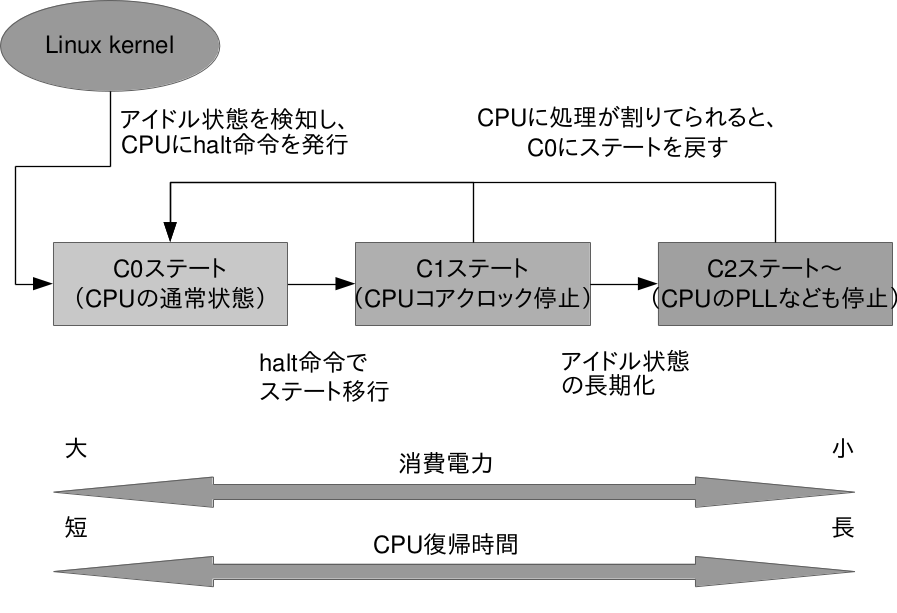
\includegraphics[width=0.5\hsize]{image201602/cpustate_mono.png}
\end{center}
\caption{CPU状態遷移簡易図} 
\label{fig:cpustate}
\end{figure}

実際のCPUはCステートだけではなく、CPUの電圧やクロック数なども関連してきます。
Linux の場合はCPU周波数スケーリング機能を使うことで、OSが自動的に制御できるようになっています。
これは Linux カーネルの cpufreq によって実装されています。
現在の cpufreq に設定されている内容を確認するには cpufrequtils パッケージで提供されている
cpufreq-info(\fgref{fig:cpufreq-info}) コマンドを使います。

\begin{figure}[htbp]
\begin{commandline}
$ cpufreq-info
cpufrequtils 008: cpufreq-info (C) Dominik Brodowski 2004-2009
Report errors and bugs to cpufreq@vger.kernel.org, please.
analyzing CPU 0:
  driver: intel_pstate
  CPUs which run at the same hardware frequency: 0
  CPUs which need to have their frequency coordinated by software: 0
  maximum transition latency: 0.97 ms.
  hardware limits: 800 MHz - 2.90 GHz
  available cpufreq governors: performance, powersave
  current policy: frequency should be within 800 MHz and 2.90 GHz.
                  The governor "powersave" may decide which speed to use
                  within this range.
  current CPU frequency is 1.90 GHz.
....
\end{commandline}

\caption{cpufreq-info 実行結果}
\label{fig:cpufreq-info}
\end{figure}

いくつか項目がありますが、重要となるのは 「available cpufreq governors」と
「current policy」です。
available cpufreq governors は CPUの調整可能な速度調整名(ガバナー)であり、
\tbref{tab:governors}が用意されています。

\begin{table}[htb]
\begin{center}
\begin{tabular}{l|l}
ガバナー & 内容 \\
ondemand &	CPU負荷が大きい、または小さい時にCPUクロックを大きくに切り替える \\
conservative &	CPU負荷が大きい、または小さい時にCPUクロックを徐々に切り替える \\
performance &	最大周波数でCPUを動作させる \\
powersave &	最小周波数でCPUを動作させる \\
userspace &	ユーザーが指定した周波数でCPUを動作させる \\
\end{tabular}
\caption{指定できるガバナー}
\label{tab:governors}
\end{center}
\end{table}

これらは実際には設定できる値カーネルや環境によって異なる点に注意が必要です。
「current policy」は現在設定されているガバナーが表示されます。

この以上から、上記の結果では

\begin{itemize}
\item CPUが800MHzから2.90GHzまでをサポートしている
\item powersave governor で動作している
\item 最大値と最小値のポリシー設定により、800MHzから2.90GHzの間で変動させている
\end{itemize}

ということがわかります。

これらを設定するには sysfs 経由で操作するか、cpufrequtils に含まれる
cpufreq-set コマンドを使います。

\begin{itemize}
\item ガバナーを設定する
  \begin{commandline}
   $ sudo cpufreq-set -c CPU番号 -g ガバナー名
   または
   $ sudo sh -c "echo ガバナー名 > /sys/devices/system/cpu/cpuCPU番号/cpufreq/scaling_governor"
  \end{commandline}

\item 最小クロックを設定する
  \begin{commandline}
   $ sudo cpufreq-set -c CPU番号 -d クロック値
   または
   $ sudo sh -c "echo クロック値 > /sys/devices/system/cpu/cpuCPU番号/cpufreq/scaling_min_freq"
  \end{commandline}

\item 最大クロックを設定する
  \begin{commandline}
   $ sudo cpufreq-set -c CPU番号 -u クロック値
   または
   $ sudo sh -c "echo クロック値 > /sys/devices/system/cpu/cpuCPU番号/cpufreq/scaling_max_freq"
  \end{commandline}

\item 現在のクロックを設定する
  \begin{commandline}
   $ sudo cpufreq-set -c CPU番号 -f クロック値
   または
   $ sudo sh -c "echo クロック値 > /sys/devices/system/cpu/cpuCPU番号/cpufreq/scaling_cur_freq"
  \end{commandline}

\end{itemize}

上記のようにしてCPUクロックを制御することにより、環境によって無駄なくCPUを利用できるようになります。
設定した値は再起動すると消えるので、/etc/sysfs.conf に設定しておくか、cpufreq を設定するデーモン cpufreqd
を使うとよいでしょう。

\subsubsection{動作しているデバイスの設定}

使っている個々のデバイスの設定も重要となります。例えば無線LANやBluetoothを使わないのに有効にしていると
それだけで電力を消費してしまいます。よって使用する環境に応じてこれらを制御する必要が出てきます。

ここではよく利用されるデバイスに対する制御方法について説明します。

\begin{itemize}

\item ラップトップモード

Linux の場合はカーネルのモードとして、ラップトップモードが設定できるようになっています。
これは以下のようにして設定します。

\begin{commandline}
$ sudo sh -c "echo 5 > /proc/sys/vm/laptop_mode"
\end{commandline}

あとNMI のwatchdog(nmi\_watchdog) も無効化しておきます。これはこれはカーネルハングアップを定期的にチェックする機構
をコントロールするフラグです。

\begin{commandline}
$ sudo sh -c "echo 0 > /proc/sys/kernel/nmi_watchdog"
\end{commandline}

\item USB

USB は /sys/bus/usb/devices/ 以下に対して設定を行います。
例えば、/sys/bus/usb/devices/usb1 に対して 電源供給を切りたい場合は /sys/bus/usb/devices/usb1/power/control
をoff に設定します。自動的にサスペンドさせたい場合には 
/sys/bus/usb/devices/usb1/power/autosuspend に対して 1 を設定します。

\begin{commandline}
$ sudo sh -c "echo off > /sys/bus/usb/devices/usb1/power/control"
$ sudo sh -c "echo auto > /sys/bus/usb/devices/usb1/power/autosuspend"
\end{commandline}

設定を起動時に適用したい場合は、再起動時に初期化されてしまう事とデバイスのUSB位置が変わる事が
ありますので、 udev の rules ファイルを使って設定するのがよいでしょう。

\begin{commandline}
実際は一行
$ cat /etc/udev/rules.d/70-my-usb-power.rules
ACTION=="add", SUBSYSTEM=="usb", ATTRS{idVendor}=="0x046d",
 ATTR{idProduct}=="0x08cb", TEST=="power/control", ATTR{power/control}="off"
\end{commandline}

注意しなければいけない点としてはUSBをなんでも設定してしまうとキーボードが動作しなくなる可能性もあるため、
ベンダーID、デバイスIDなどを確認した上で設定しましょう。

\item 無線LAN

無線LANは iw パッケージに含まれる iw コマンドを使って設定します。
無線LANがwlan0の場合は 以下のように設定することによって制御できます。

\begin{commandline}
$ sudo iw dev wlan0 set power_save on
\end{commandline}

これもudev の rules ファイルを使って設定すると良いです。

\begin{commandline}
$ cat /etc/udev/rules.d/70-my-wifi-power.rules
ACTION=="add", SUBSYSTEM=="net", KERNEL=="wlan*", RUN+="/usr/bin/iw dev %k set power_save on"
\end{commandline}

\item サウンド

サウンドの場合も sysfs 経由で設定します。ドライバによって設定出来ない場合がありますが、INTEL のサウンド
コントローラの場合は、power\_save があるので、これを1に設定することによってパワーセーブモードに設定できます。

\begin{commandline}
$ sudo sh -c "echo 1 > /sys/module/snd_hda_intel/parameters/power_save"
\end{commandline}

\item PCI/PCI-Express

PCI/PCI-Express の省電力に設定するには power/control を auto に設定します。
この場合も sysfs 経由で設定します。PCIもUSBと同様に設定先がどのようなデバイス
なのか確認してから設定するようにしましょう。

\begin{commandline}
$ sudo sh -c "echo auto > /sys/bus/pci/devices/0000:00:00.0/power/control"
\end{commandline}

\end{itemize}

\subsubsection{動作しているプログラムについて}

動作しているプログラムはtopコマンドなのでざっくりとしたCPU占有率を確認できますが、実際に
どれぐらいの頻度で使われてているのかわかりません。アイドル状態であるにもかかわらず、CPU割り込みが多い
プログラム・プロセスが省電力の効果が得にくいものとなりますので、このようなプログラム・プロセスを
調べる必要があります。これらを調べるには下記で説明する PowerTop を使うとようでしょう。

\subsection{省電力設定するためのツール}

先では長々と書きましたが、知識がないユーザが上記を一つづつやっていくのは非常に大変です。
Linux では専門の知識がなくとも使っているマシンを省電力状態に設定できるツールがいくつか
準備されています。以下ではそれらの使い方について紹介します。

\subsubsection{PowerTOP}

PowerTOP はIntelが開発しているソフトウェアで、カーネル、ハードウェア、ユーザランドで制御可能な省電力項目を
有効にするツールです。プロセスを監視して、CPU負荷やデバイスドライバの使用状況のレポートからプロセスの操作
を行う事ができます。

\begin{enumerate}

\item インストール

PowerTOP はDebian でも提供されており、apt でインストールできます。
\begin{commandline}
$ sudo apt-get install powertop
\end{commandline}

\item 起動

起動すると\fgref{fig:powertop0}のような画面が表示されます。
「The battery reports a discharge rate ...」 に現在の消費電力が
表示され、現在動作しているプロセスと使用状況がわかります。
筆者の環境で、何も設定しない場合は 13Wのようです。

\begin{figure}[H]
\begin{center}
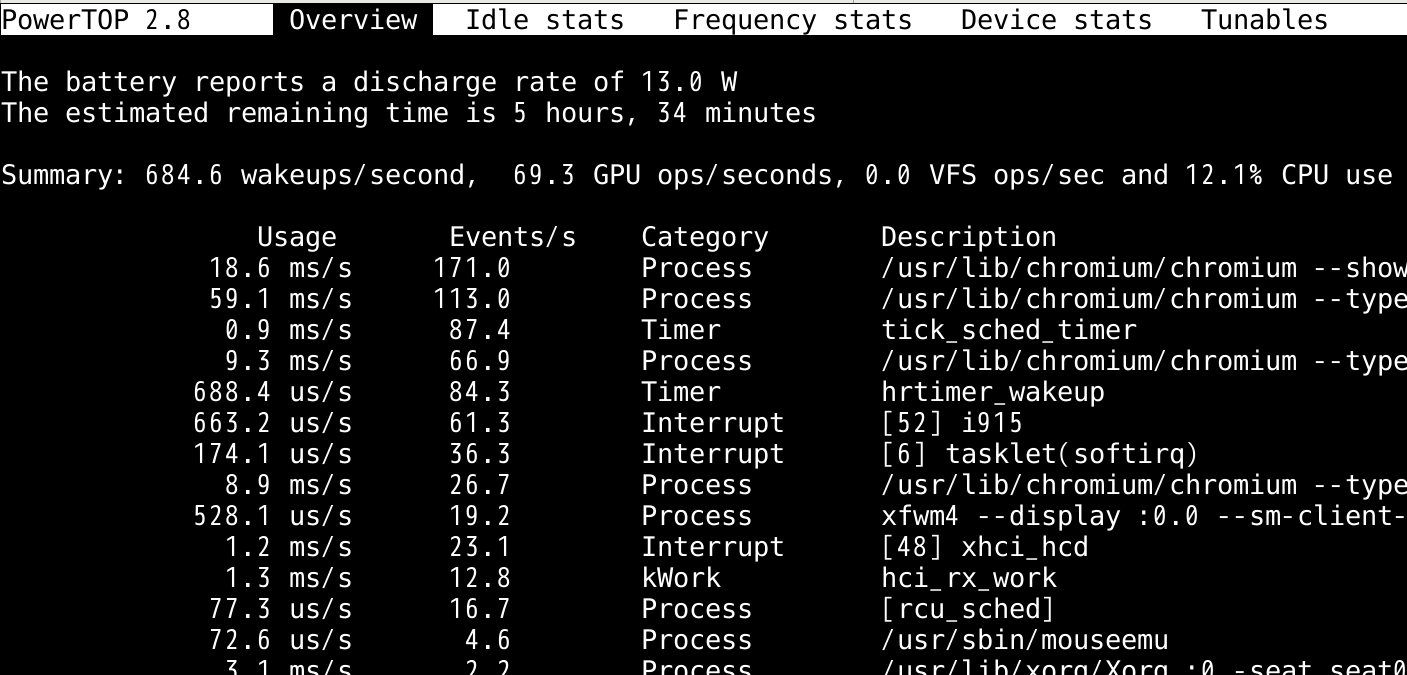
\includegraphics[width=0.5\hsize]{image201602/powertop_00.png}
\end{center}
\caption{PowerTOP起動画面} 
\label{fig:powertop0}
\end{figure}

Tunables タブを選択すると調整可能なシステムの設定が表示されます(\fgref{fig:powertop1})。
Badが省電力に有効な項目にもかかわらず無効な設定、
Good が既に有効になっている設定となっています。

\begin{figure}[H]
\begin{center}
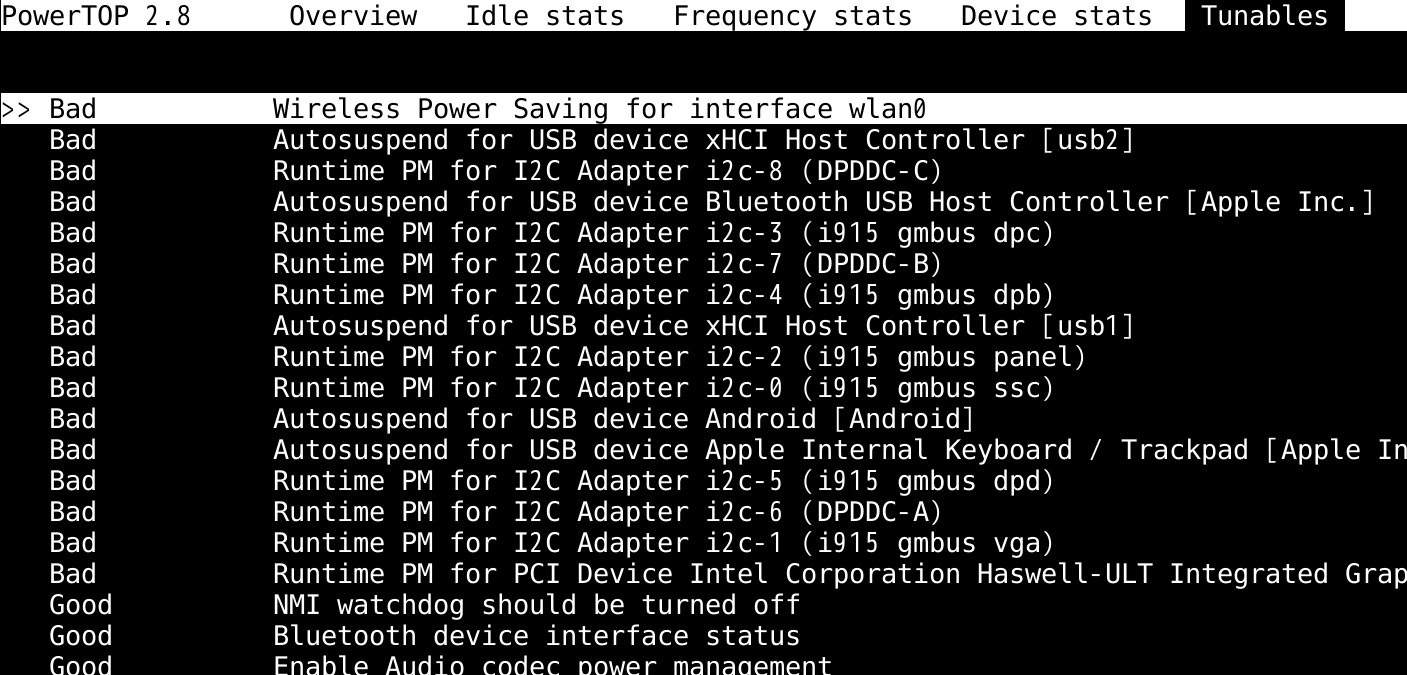
\includegraphics[width=0.5\hsize]{image201602/powertop_01.png}
\end{center}
\caption{Tunables画面} 
\label{fig:powertop1}
\end{figure}

この状態ではまだシステムに最適化された設定になっていないため、一度終了し、
キャリブレーションを行います。

\item キャリブレーション

設定するPCの状態を取得するためにキャリブレーションを行います。
実行するとデバイスなどから使用状況を読み取り、マシンに対して適切な設定を
行います。
ノートPCの場合はいきなりモニターのバックライトが消えるので注意しましょう。

\begin{commandline}
$ sudo powertop --calibrate
\end{commandline}

キャリブレーションが終わると、\texttt{/var/cache/powertop/saved\_parameters.powertop}
以下にデータが保存されます。次回のPowerTOP起動時からはキャリブレーションデータを元に
省電力にされた環境で起動します。

\item キャリブレーション後

キャリブレーション後に起動すると、
「The battery reports a discharge rate ...」 の項目に表示される消費電力値が変わり、システム
全体で省電力で稼働していることが確認できるでしょう。

\item PowerTOP の起動時有効化

PowerTOP は起動すると保存されている設定を元に省電力状態にしてくれますが、PCを立ち上げるたびに
PowerTOP自体を立ち上げる必要があります。

起動時に自動的にPowerTOP を立ち上げるようにするには、以下のように systemd の ユニットファイル
を用意し、有効にしておきます。

\begin{commandline}
$ cat /etc/systemd/system/powertop.service

[Unit]
Description=PowerTOP

[Service]
Type=oneshot
ExecStart=/usr/bin/powertop
Environment="TERM=xterm"

[Install]
WantedBy=multi-user.target
\end{commandline}

\begin{commandline}
$ sudo systemctl enable powertop
\end{commandline}

\end{enumerate}

\subsubsection{TLP を使った設定}

PowerTOP の他にTLPというツールもあります。これは PowerTOPのように詳細なレポートは
出してくれませんが、AC接続時などの状況に応じたスクリプトが準備されており、インストール
するだけである程度省電力設定を行ってくれる便利なツールです。
もちろん、Debian ではパッケージ化されており、apt でインストールできます。

\begin{commandline}
$ sudo apt-get install tlp
\end{commandline}

無線LANの設定等に NetworkManager を使っているなら tlp-rdw パッケージもインストールしておくと
無線LAN、Bluetooth関連の設定も行ってくれます。
デフォルトの設定は /etc/default/tlp にあり、このファイルを変更して環境に合わせた省電力設定を
行います(\fgref{fig:TLP})。設定はよく使われる項目しかなく、使っている環境の設定がない場合もあります。このような場合は
T自分で設定を追加するか、先に説明したようにsysfs / procfs 経由
の設定を別途行う必要があります。


\begin{figure}[H]
\begin{center}
\begin{commandline}
# Set to 0 to disable, 1 to enable TLP.
TLP_ENABLE=1

# Operation mode when no power supply can be detected: AC, BAT
# Concerns some desktop and embedded hardware only.
TLP_DEFAULT_MODE=AC

# Seconds laptop mode has to wait after the disk goes idle before doing a sync.
# Non-zero value enables, zero disables laptop mode.
DISK_IDLE_SECS_ON_AC=0
DISK_IDLE_SECS_ON_BAT=2

# Dirty page values (timeouts in secs).
MAX_LOST_WORK_SECS_ON_AC=15
MAX_LOST_WORK_SECS_ON_BAT=60
...
\end{commandline}
\end{center}
\caption{/etc/default/tlp 例} 
\label{fig:TLP}
\end{figure}

TLP は systemd やその他init用の起動ファイルが用意されているのでPC起動時に設定が反映されるのも
良い点です。

\subsubsection{省電力設定後}
\fgref{fig:powertop2}が省電力設定した後に PowerTOP で消費電力を確認した内容です。
消費電力が13W から 11W に下がっていることがわかります。またPC稼働時間も5時間半から6時間50分に
伸びていることがわかります。

\begin{figure}[H]
\begin{center}
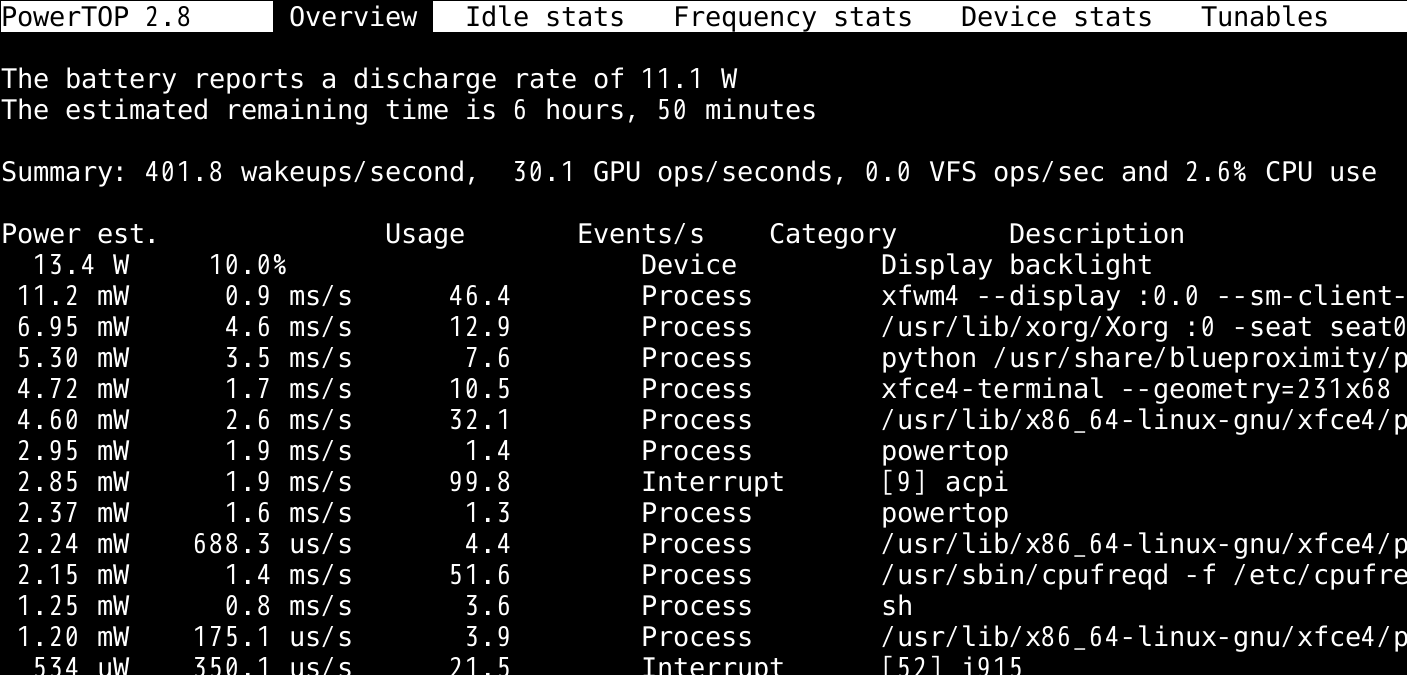
\includegraphics[width=0.5\hsize]{image201602/powertop_02.png}
\end{center}
\caption{省電力設定後} 
\label{fig:powertop2}
\end{figure}

\subsection{まとめ}

Debian での省電力設定について説明しました。
現在の状態をとりあえず確認するには cpufreq-info を使い、カーネルの設定やドライバの設定は
sysfs や proc fs 経由で設定します。プログラムやプロセスの詳細な状態の確認するには PowerTOP
を使います。省電力設定できる項目もわかり、ユーザインターフェイスから各種設定ができるようになっています。
また再立ち上げすると省電力設定を再設定する必要がありますので、sysytem用のservice
ファイルを別途用意するなどの対策が必要です。
細かい設定を行わなくても、とりあえず省電力設定を行いたい場合はTLPを使うのがよいでしょう。ただ全ての
PCをサポートしているわけではありませんので、環境に合わせてプログラムを修正するなりの対応が必要となります。

\dancersection{LibreOfficeの最近の動向とDebianでのLibreOfficeパッケージについて}{榎 真治}

\subsection{2015年のLibreOfficeを振り返って}
\begin{itemize}
\item %
LibreOffice Online(LOOL)の開発が本格開始
\item %
LibreOffice Viewerリリース
\item %
編集機能は実験的な段階
\item %
開発/リリースも順調に
\item %
機能面以外でも、UXの改善に取り組み
\item %
相互運用性(フィルタ)の改善
\item %
2015年9月には5周年!
\end{itemize}

\subsection{LibreOffice Online}
\begin{itemize}
\item %
まだまだ開発中
\item %
UIがHTML5、ブラウザで編集する
\item %
複数ユーザーの同時編集
\item %
サーバープログラムとして提供
\item %
誰でもサーバーをたてられる
\item %
ホスティングサービスも出てくるのでは
\item ownCloudの編集画面でLOOLを使うデモ
\url{https://www.youtube.com/watch?v=jPGBRu085Dw}
\end{itemize}

\subsection{プロジェクトの状況}
\begin{itemize}
\item %
Advisory Board(現在webでは17)
\item %
CIB, ミュンヘン市,Rusbitechがこの1年で参加
\item %
アクティブなコミッターは毎月100人程度
\item %
TDFのスタッフは6名(メンバー211名)
\item %
TDFメンバー以外でもアクティブな人は多い
\item %
ヨーロッパでは行政中心に導入が進行中
\item %
イタリア国防省15万台
\item %
フランス内務省24万台(これは以前から)
\item %
イギリス政府もODF 標準、Collaboraとも契約しLibreOffice導入へ
\item %
台湾もODF推進、自治体でLibreOffice導入
\end{itemize}

\subsection{今年の日本での活動}
\begin{itemize}
\item %
翻訳
\item %
UIの翻訳率は高い,Helpはますます追いついてない\\
(翻訳率は高くても誤訳を見つけて修正しきれてない、とのツッコミあり)
\item %
英語のHelpも実装に追いついてないケースも
\item %
ドキュメント系翻訳はアナウンスくらい
\item %
翻訳査読スプリントを開催(査読が溜まってきていた+ルールの議論)
\item %
品質保証
\item %
HackFest (Bugハンティング)7回
\item %
クラッシュバグなどいくつか発見/レポート
\end{itemize}

\subsection{今年の日本での活動2}
\begin{itemize}
%\item %
%イベント
\item %
日本語コミュニティのイベント+ブース出展など46回
\item %
HackFest を増やした(10回)、来年も重点的に
\item %
QAなど集まってやることで作業がやりやすかった
\item %
まだまだ参加者は少ない
\item %
開発向けも1回、LibreOfficeのビルドネタで挑戦
\item %
関西LibreOffice HackFest 2015-08-22(開発)
\item %
LibreOffice Hackfest (翻訳査読スプリント) 2015-07-26 in 東京
\end{itemize}

\subsection{LibreOffice Conference 2015}
\begin{itemize}
\item %
開催地:デンマーク・オーフス
\item %
日時:2015/9/23(水)-25(金)
\item %
約80のセッション
\item %
参加者:約150名
\item %
例年より多め、アジア勢も増えた
\item %
日本からは3名
\item %
小笠原さん、山本さん、榎
\item %
NLPワークショップ
\item %
ITProでのカンファレンスレポート\url{http://itpro.nikkeibp.co.jp/atcl/column/15/102800252/}
\end{itemize}

%とりとめない部分なので、省略
%\subsection{各言語のコミュニティ}
%\item %
%LibreItalia(非営利団体)
%\item %
%教育向けも活発:教師向け、保護者向け、子供向け
%\item %
%ベトナムコミュニティ
%\item %
%物理的な距離が離れている。ルール作りをした
%\item %
%MSOは英語UIしかないが、何をどこまで翻訳するか?
%\item %
%LibreOfficeだけをやっている人はほぼいない
%\item %
%複数のコミュニティをかけもち
%\item %

%開催後なのでレポートベースの資料で更新
\subsection{LibreOffice mini Conference 2016 in Japanを開催しました}
\begin{itemize}
\item %
日時:2016/1/9(土) 13:00-18:00
\item %
場所:GMO Yours!(グランフロント大阪)
\item %
参加者:48名
\item %
ITProでのカンファレンスレポート\url{http://itpro.nikkeibp.co.jp/atcl/column/14/090100053/013100122/}
\end{itemize}

\subsection{DebianでのLibreOfficeパッケージ}

TDFで提供されているソースコードをTDF版、
Debianでapt-get sourceで取得できるソースコードをDebian版と、この資料では呼ぶことにします
\subsection{TDF版のソースを落としてみる}
\begin{commandline}
$ tar -Jxvf libreoffice-4.3.3.2.tar.xz 
$ du -h libreoffice-4.3.3.2
931M libreoffice-4.3.3.2
\end{commandline}
Debian版のソースを取得する
Debianパッケージのソースを取得する(環境:安定版jessie)
\begin{commandline}
$ sudo aptitude install dpkg-dev
$ apt-get source libreoffice

$ ls -lh
drwxr-xr-x 153 eno eno  48K 12月 26 21:06 libreoffice-4.3.3
-rw-r--r--   1 eno eno 2.1M  9月  5 03:25 libreoffice_4.3.3-2+deb8u2.debian.tar.xz
-rw-r--r--   1 eno eno  26K  9月  5 03:25 libreoffice_4.3.3-2+deb8u2.dsc
-rw-r--r--   1 eno eno 308M  4月  9  2015 libreoffice_4.3.3.orig-external.tar.xz
-rw-r--r--   1 eno eno 1.4M  4月  9  2015 libreoffice_4.3.3.orig-helpcontent2.tar.xz
-rw-r--r--   1 eno eno 122M  4月  9  2015 libreoffice_4.3.3.orig-translations.tar.xz
-rw-r--r--   1 eno eno 143M  4月  9  2015 libreoffice_4.3.3.orig.tar.xz
\end{commandline}
\subsection{externalは、他のOSSのこと}
\begin{itemize}
\item %
Debian版は、他のOSS本体のソースコードを含む
”external/tarballs/”以下
Python3, hsqldb, poppler, 各種フォントなど大量に
\item %
TDF版は、他のOSSへのパッチのみ
初めてmakeする時に他のOSSの本体はダウンロード
なので1回目のビルドは結構時間がかかる
\end{itemize}
\subsection{ファイル一覧のdiff(Debian版にしかないもの)}
\begin{commandline}
/.pc/ 以下745 .pc/以下はquiltのDebian向け修正記録 
/bridges/ 以下7
/translations/以下 TDF版は翻訳、ヘルプは別になっている
/helpcontent2/以下
/debian/以下131 debian/以下はdebian独自パッチ
/external/tarballs/以下109
/solenv/gbuild/platform/LINUX_AARCH64_GCC.mk それ以外に、3ファイルほど追加されている...
/writerfilter/qa/cppunittests/rtftok/data/pass/sf_2063317381c4a46d642c79a4b1817dc0-101375-minimized.rtf
/writerfilter/qa/cppunittests/rtftok/data/pass/sf_2063317381c4a46d642c79a4b1817dc0-108116-minimized.rtf
\subsection{libreoffice-4.3.3のディレクトリ構成}
$ du -h libreoffice-4.3.3/
...
2.7G libreoffice-4.3.3/
内、translations/以下が1.5Gと大きな割合を占める

$ cd libreoffice-4.3.3/
$ du -h debian/
4.0K	debian/pyuno-for-2.7
44K	debian/scripts
488K	debian/patches
12K	debian/source
8.0K	debian/branding
12K	debian/tests/patches
24K	debian/tests
2.9M	debian/templates
8.0K	debian/upstream
5.0M	debian/
\end{commandline}
\subsection{libreoffice-4.3.3/debian/patches/に含まれるファイル}
\begin{itemize}
\item %
46のパッチファイル
\item %
セキュリティFIXのパッチは6つ、セキュリティFIXは対応できているよう
\footnote{\url{https://www.libreoffice.org/about-us/security/advisories/}}
\item %
libreofficeのmasterから取り込み6つ程度、それ以外のmasterから取り込みもある
\item %
その他、Debianの設定やビルド周りのパッチで
(ざっとみた感じでは)Debian独自の機能はなさそう
\end{itemize}

%Debian での変更履歴
%\begin{commandline}
%backport-rtf-fixes.diff (CVE-2014-9093)
%Bug 86449 - Crash importing malformed .rtf
%\end{commandline}

\subsection{DebianのLibreOfficeバージョン(2015年12月時点)}
\begin{itemize}
\item %
experimental: 現在 1:5.1.0~rc1-1
LibreOfficeの開発版。5.1系Alpha → Beta →リリース候補(RC)
\item %
sid(stretchも同じ): 現在 1:5.0.4~rc2-2
LibreOfficeの最新版(fresh)のリリース候補とリリース版
\item %
jessie(Stable) : 現在 1:4.3.3-2+deb8u2
2回アップデート (2015/3/26: CVE-2015-1774, 2015/8/28 : CVE-2014-4551,VE-2015-5213,CVE-2015-5212,CVE-2015-5214)
sid時代に1回セキュリティFIX (2014/11/27 : CVE-2014-9093)
\item %
jessie-backports: 現在 1:5.0.4~rc2-2
LibreOfficeの最新版(fresh)とそのリリース候補
安定版(jessie)でもLibreOfficeの最新版が利用できる
\end{itemize}
\begin{center}
Enjoy Debian and LibreOffice Life!
\end{center}

\subsection{著者紹介}
\begin{itemize}
\item %
榎真治(えのきしんじ)
\item %
LibreOffice日本語チームメンバー(2011-現在)
主にイベント担当、2015年はLibreOfficeコミュニティイベント34回くらい開催/参加
%\item %
%今日みたいなのはカウント外です
\item %
The Document Foundationメンバー(2014/4-現在)
\item %
フリーでLibreOfficeのコンサル/サポート/トレーニング
\item %
アイクラフト株式会社と組んでLibreOfficeサポートビジネス
(CollaboraのサポートのリセールとL1/L2サポート)を開始
\end{itemize}

%201512
\dancersection{Debian モバイル wifi ルータ化}{野島 貴英}

\subsection{はじめに}

 最近のモバイルルータは、7GBytes/月、300MBytes/日などの、一定の通信量を超えるとたちまち通信制限がかかってしまい、とても実用にならないぐらいに通信帯域を絞られてしまいます。
  
 たまたま、手元に通信制限が非常にゆるい(というか気にならない)FOMAのモデムがありましたので、こちらとDebianを使ってモバイルルータが作れないかを試してみました。また、Linuxで無線APを作る時の仕組みについてもちょっと調べてみました。
 


\subsection{用意するもの}

  用意するものは次のとおり。

  \begin{itemize}
  \item Debianの動くモバイルPC
  \item DoCoMo社 L-05A (モデム。データ定額制の契約であること。)
  \item BUFFALO WLI-UC-GNM2 (備考:Ralink製 Ralink RT3070搭載。900円/1個ぐらいの小型USB無線LANアダプタ)
  \end{itemize}    



\subsection{bridgeを作る}

  \begin{description}
    \item [Step 1-1] apt install bridge-utils
    \item [Step 1-2] vi /etc/network/interfaceして以下を追記
  \end{description}      
 /etc/network/interfaceの追記部分:
\begin{commandline}
auto br0
iface br0 inet static
        address 192.168.0.1
        netmask 255.255.255.0
        bridge_ports none
        bridge_stp off
        bridge_fd 0
        bridge_maxwait 0
\end{commandline}

  \begin{description}
    \item [Step 1-3] ifup br0
    \item [Step 1-4] vi /etc/sysctl.d/bridge-filter-workaround.conf
  \end{description}      
/etc/sysctl.d/bridge-filter-workaround.conf中身:
\begin{commandline}
net.bridge.bridge-nf-call-ip6tables = 0
net.bridge.bridge-nf-call-iptables = 0
net.bridge.bridge-nf-call-arptables = 0
\end{commandline}

  \begin{description}
    \item [Step 1-5] vi /etc/sysctl.d/forward-yes.conf
  \end{description}      
 /etc/sysctl.d/forward-yes.conf中身:
\begin{commandline}
net.ipv4.ip_forward=1
\end{commandline}

  \begin{description}
  \item [Step 1-6] sysctl -p /etc/sysctl.d/bridge-filter-workaround.conf
  \item [Step 1-7] sysctl -p /etc/sysctl.d/forward-yes.conf
 \end{description}

\begin{figure}[htbp]
\includegraphics[width=0.5\hsize]{image201512/bridge.eps}
\caption{bridgeの設定の状況}
\end{figure}
  
\subsection{L-05A側設定}

  \begin{description}
    \item [Step 2-1] apt install ppp
    \item [Step 2-2] vi /etc/ppp/peers/l-05a
  \end{description}      


 /etc/ppp/peers/l-05aの中身:
\begin{commandline}
hide-password 
noauth 
connect "/usr/sbin/chat -v -f /etc/chatscripts/l-05a"
debug 
/dev/ttyACM0
115200
defaultroute
noipdefault 
user ""
remotename l-05a
ipparam l-05a
persist 
usepeerdns 
idle 300
\end{commandline}
  
  \begin{description}
    \item [Step 2-3] vi /etc/chatscripts/l-05a
  \end{description}      
 /etc/chatscripts/l-05aの中身:
\begin{commandline}
ABORT BUSY ABORT 'NO CARRIER' ABORT VOICE 
ABORT 'NO DIALTONE' ABORT 'NO DIAL TONE' 
ABORT 'NO ANSWER' ABORT DELAYED
'' ATZ
OK-AT-OK "ATDT*99***5#"
CONNECT \d\c
\end{commandline}

  \begin{description}
    \item [Step 2-4] chown root:dip /etc/ppp/peers/l-05a /etc/chatscripts/l-05a
    \item [Step 2-5] chmod 640 /etc/ppp/peers/l-05a /etc/chatscripts/l-05a
    \item [Step 2-6] vi /etc/ppp/ip-up.d/bridge-up
  \end{description}      
 /etc/ppp/ip-up.d/bridge-upの中身:
\begin{commandline}
#!/bin/sh
iptables -t nat -A POSTROUTING -o $PPP_IFACE \
-j MASQUERADE
iptables -A FORWARD -i br0 -o $PPP_IFACE -j ACCEPT
iptables -A FORWARD -o br0 -i $PPP_IFACE -j ACCEPT
\end{commandline}

  \begin{description}
    \item [Step 2-7] vi /etc/ppp/ip-down.d/bridge-down
  \end{description}      
 /etc/ppp/ip-down.d/bridge-downの中身:
\begin{commandline}
#!/bin/sh
PATH=/bin:/usr/bin:/sbin:/usr/sbin
iptables -t nat -D POSTROUTING -o $PPP_IFACE \
-j MASQUERADE
iptables -D FORWARD -i br0 -o $PPP_IFACE -j ACCEPT
iptables -D FORWARD -o br0 -i $PPP_IFACE -j ACCEPT
\end{commandline}

  \begin{description}
    \item [Step 2-8] chown 755 /etc/ppp/ip-up.d/bridge-up /etc/ppp/ip-up.d/bridge-down
    \item [Step 2-9] pon l-05a
  \end{description}      
 これで、L-05aはグローバルに接続されるようになります。

\begin{figure}[htbp]
\includegraphics[width=0.5\hsize]{image201512/pppd.eps}
\caption{pppの設定の状況}
\end{figure}

\subsection{補足:L-05A側トラブルシュート}

 つながらない時は次のとおりです。

 \begin{itemize}
 \item tail -f /var/log/debug /var/log/messagesに詳細なログが出ます。こちらを見ると解決のためのヒントが見つかります。
 \item pon l-05aをした後、ttyACM0が見つからないというエラーが出ることがあります。この場合は、次の手続きを取ると治ります。\\
 modprobe -r uas;modprobe uas;eject /dev/sr0
 \end{itemize} 



\subsection{hostapdの設定}

  いよいよ無線APを立てます。

  \begin{description}
  \item [Step 3-1] apt install hostapd firmware-ralink
  \item [Step 3-2] ここで、WLI-UC-GNM2をPCに差し込む。
  \item [Step 3-3] lsmodして以下のモジュールがロードされたことを確認。
  \end{description}      
 lsmodの結果抜粋
\begin{commandline}
rt2800usb              28672  0
rt2x00usb              24576  1 rt2800usb
rt2800lib              90112  1 rt2800usb
rt2x00lib              53248  3 rt2x00usb,rt2800lib,
                                rt2800usb
mac80211              630784  4 rt2x00lib,rt2x00usb,
                                rt2800lib
cfg80211              532480  4 mac80211,rt2x00lib
rfkill                 24576  5 cfg80211
\end{commandline}



\subsection{hostapdの設定}

  \begin{description}
  \item [Step 3-4] ip addr showして、wlxXXXXXXXXXXXXという名前のI/Fを探す。
  \item [Step 3-5] vi /etc/hostapd/hostapd.conf
  \end{description}      

/etc/hostapd/hostapd.confの中身:
\begin{commandline}
interface=wlxXXXXXXXXXXXX 
bridge=br0
driver=nl80211
hw_mode=g
ieee80211n=1
ssid=debianspot
wpa_passphrase=abcdef
macaddr_acl=0
wpa=2
channel=1
wpa_key_mgmt=WPA-PSK
wpa_pairwise=CCMP
logger_syslog=-1
logger_syslog_level=2
ctrl_interface=/var/run/hostapd
\end{commandline}


\subsection{hostapdの設定}

  \begin{description}
  \item [Step 3-6] chmod 600 /etc/hostapd/hostapd.conf
  \item [Step 3-7] systemctl start hostapd.service
  \end{description}      

  これで無線APが稼働します。iphone/Android端末で見ると、SSID: debianspotというSSIDが見えるはずです。ただ、まだ、dhcpサービスを有効にしていないため、パスワードを入れても接続できません。

\begin{figure}[htbp]
\includegraphics[width=0.5\hsize]{image201512/hostapd.eps}
\caption{hostapd稼働の状況}
\end{figure}

\subsection{DHCPの設定}

  今回簡易的にdhcpサーバを立てるため、dnsmasqを利用します。
  \begin{description}
  \item [Step 4-1] apt install dnsmasq
  \item [Step 4-2] vi /etc/dnsmasq.d/dhcp.conf
  \end{description}      

dhcp.confの中身:
\begin{commandline}
interface=br0
bind-interfaces
dhcp-range=192.168.2.129,192.168.2.254,
255.255.255.0,1h
\end{commandline}
  

  \begin{description}
  \item [Step 4-3] systemctl start dnsmasq.service
  \end{description}      

  以上で、dhcpサービスがbr0経由で開始され、無事、無線APとして稼働します。iphone/AndroidからもSSID: debianspotに接続し、パスワード'abcdef'を入れると、WPA2-PSKにて接続されます。
  

\begin{figure}[htbp]
 \begin{minipage}{0.5\hsize}
\includegraphics[width=0.9\hsize]{image201512/dhcp.eps}
\caption{無線AP稼働の状況}
 \end{minipage}
 \begin{minipage}{0.5\hsize}
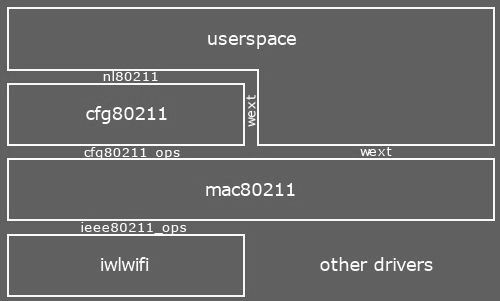
\includegraphics[width=0.9\hsize]{image201512/mac80211_arch_mono.jpg}
\caption{nl80211の図示}
 \end{minipage}
\end{figure}

\subsection{hostapdはどのようにWLI-UC-GNM2を操作するのか?}


  cfg8011とhostapdは通信をしてWLI-UC-GNM2を操作するのですが、こちらで使われる
 プロトコルは、linuxのNETLINKが利用されます。



%201601 kansai
\dancersection{VyOSを入れてAPを構築してみた。}{かわだてつたろう}

\subsection{VyOS}

VyOS\footnote{\url{http://vyos.net}}はLinuxベースのネットワークオペレーティングシステムです。
ルーティング、ファイヤーウォール、VPNの構築に使用されています。

元々はVyatta社が開発していたVyatta Coreでしたが開発元が買収された後に提供が終了したため、
ここからフォークし開発が開始されたのがVyOSになります。

VyOSはDebianをベースにしており、最新リリースのVyOS 1.1.6 (Helium)は
Debian 6 Squeezeがベースとなっています。

\subsection{初期設定}

インストーラのISOイメージはLive CDとして提供されていますのでUser GuideのInstallation
\footnote{\url{http://vyos.net/wiki/User_Guide\#Installation}}
の手順通りにインストールを進めます。

続いてルータとして使用するための設定を行ないます。ここではUser GuideのQuick Start Guide
\footnote{\url{http://vyos.net/wiki/User_Guide\#Quick_Start_Guide}}
の通りに設定します。
これで外と内(192.168.0.1/24)を繋ぐルータができあがります。

\subsection{アクセスポイントの構築}

アクセスポイントに使用する無線LANアダプタとして
{\tt en:users:drivers [Linux Wireless]}
\footnote{\url{https://wireless.wiki.kernel.org/en/users/drivers}}
を参考に、Linuxが対応しており、アクセスポイントとして動作するアダプタを用意します。

今回はAtheros製のAR9280を使います。

このアダプタを先に設定した内側のネットワークに追加する形でアクセスポイントを設定
します。

手順としてはブリッジを作成しそこに内側のインターフェース(eth0)と
無線LANのインターフェース(wlan0)を追加します。この際追加するイン
ターフェースにaddressが設定されているとエラーになりますので先に
削除します。
\footnote{\url{http://orebibou.com/2015/01/apu1-c\%E3\%81\%AB\%E7\%84\%A1\%E7\%B7\%9Alan\%E3\%82\%A2\%E3\%83\%B3\%E3\%83\%86\%E3\%83\%8A\%E3\%82\%92\%E5\%8F\%96\%E3\%82\%8A\%E4\%BB\%98\%E3\%81\%91\%E3\%81\%A6vyos\%E3\%81\%AE\%E7\%84\%A1\%E7\%B7\%9Alan\%E3\%83\%AB\%E3\%83\%BC\%E3\%82\%BF\%E3\%83\%BC/}}

\begin{commandline}
vyos@vyos:~$ configure
vyos@vyos# delete interfaces ethernet eth1 address 192.168.0.1/24
vyos@vyos# set interfaces bridge br0
vyos@vyos# set interfaces ethernet eth1 bridge-group bridge br0
vyos@vyos# set interfaces wireless wlan0 bridge-group bridge br0
vyos@vyos# set interfaces bridge br0 address 192.168.0.1/24
vyos@vyos# commit
vyos@vyos# save
\end{commandline}
%% $

続いてeth1として設定したサービスをbr0に変更しておきます。

\begin{commandline}
vyos@vyos# delete service dns forwarding listen-on eth1
vyos@vyos# set service dns forwarding listen-on br0
vyos@vyos# commit
vyos@vyos# save
\end{commandline}

そして無線LANアクセスポイントの設定を行います。

\begin{commandline}
vyos@vyos# set interfaces wireless wlan0 country JP
vyos@vyos# set interfaces wireless wlan0 mode g
vyos@vyos# set interfaces wireless wlan0 channel 10
vyos@vyos# set interfaces wireless wlan0 ssid vyos
vyos@vyos# set interfaces wireless wlan0 security wpa mode wpa2
vyos@vyos# set interfaces wireless wlan0 security wpa passphrase password
vyos@vyos# set interfaces wireless wlan0 type access-point
vyos@vyos# commit
vyos@vyos# save
\end{commandline}

これでIEEE802.11gのアクセスポイントができあがりました。

アクセスポイントに接続できない場合はアクセスポイントデーモンのhostapdが起動して
いないかdhcpdサーバがbr0を認識していないことが考えられますので、それぞれの
デーモンを再起動してください。

もしくは一度再起動しておくとよいかもしれません。

\begin{commandline}
vyos@vyos~$ sudo /opt/vyatta/sbin/hostapd-init start wlan0
\end{commandline}
%% $

\begin{commandline}
vyos@vyos~$ configure
vyos@vyos# run restart dhcp server
vyos@vyos# exit
\end{commandline}
%% $


\subsection{5GHz帯とIEEE802.11nの使用}

今回、使用した無線LANアダプタは5GHz帯とIEEE802.11nに対応していますのでこれらを使用
できるようにしてみます。

\subsubsection{IEEE802.11a}

まずは5GHz帯のIEEE802.11aの設定を行なってみます。

\begin{commandline}
vyos@vyos~$ configure
vyos@vyos# set interfaces wireless wlan0 mode a
vyos@vyos# set interfaces wireless wlan0 channel 36
vyos@vyos# commit
[ interfaces wireless wlan0 channel 36 ]
Channel 36 is not available for wlan0

[[interfaces wireless wlan0]] failed
Commit failed
[edit]
\end{commandline}
%% $

となり、設定に失敗します。

iwコマンドでチャンネルを確認すると設定したチャンネルがBand 2にあることが
確認できます。

\begin{commandline}
vyos@vyos:/opt/vyatta/sbin$ /usr/sbin/iw list
Wiphy phy0
	Band 1:

<snip>

	Band 2:
		Capabilities: 0x11ce
			HT20/HT40
			SM Power Save disabled
			RX HT40 SGI
			TX STBC
			RX STBC 1-stream
			Max AMSDU length: 7935 bytes
			DSSS/CCK HT40
		Maximum RX AMPDU length 65535 bytes (exponent: 0x003)
		Minimum RX AMPDU time spacing: 8 usec (0x06)
		HT TX/RX MCS rate indexes supported: 0-15
		Frequencies:
			* 5180 MHz [36] (15.0 dBm) (passive scanning, no IBSS)
			* 5200 MHz [40] (15.0 dBm) (passive scanning, no IBSS)
			* 5220 MHz [44] (15.0 dBm) (passive scanning, no IBSS)
			* 5240 MHz [48] (15.0 dBm) (passive scanning, no IBSS)

<snip>

\end{commandline}
%% $

これは設定スクリプトがBand 2のチャンネルを見ていないためですので、
とりあえずこの部分を潰して再度同じ設定を行ないます。

\begin{commandline}
vyos@vyos~$ configure
vyos@vyos# set interfaces wireless wlan0 mode a
vyos@vyos# set interfaces wireless wlan0 channel 36
vyos@vyos# commit
\end{commandline}
%% $

今度はエラーなく設定が完了します。しかし、アクセスポイントが表われず
hostapdデーモンも起動していません。

これは設定したチャンネルが、{\tt (passive scanning, no IBSS)}とあるように、
パッシブスキャン状態でありアクセスポイントとなることができないためです。

そこで設定スクリプトを再度修正し、パッシブスキャン状態のチャンネルも除外する
ようにします。先の修正とあわせて次のパッチのような感じになります。

\begin{commandline}
--- /opt/vyatta/sbin/wireless-config.pl.org	2016-01-23 05:09:41.455210793 +0000
+++ /opt/vyatta/sbin/wireless-config.pl	2016-01-23 05:26:43.960649746 +0000
@@ -83,10 +83,10 @@
 	while (<$iwcmd>) {
 	    chomp;
 	    next if /\(disabled\)/;
+	    next if /\(.*?(passive scanning|no IBSS).*?\)/;
 	    last unless /\* \d+ MHz \[(\d+)\]/;
 	    push @chans, $1;
 	}
-	last;
     }
     close $iwcmd;
     return @chans;
\end{commandline}
%% $

ここまでの結果では5GHz帯で使用できるチャンネルは一つもないことになります。

\subsubsection{カーネルドライバの変更}

{\tt en/users/Drivers/ath - Linux Wireless}の
{\tt 5 GHz with world regulatory domain and beacon hints}
\footnote{\url{http://linuxwireless.org/en/users/Drivers/ath/\#A5_GHz_with_world_regulatory_domain_and_beacon_hints}}
によると5GHz帯は全てパッシブスキャン状態となっているようです。

これは各国、地域ごとに使用できる周波数帯が異なるためだと思われます。
日本においても無線LANで使用する5GHz帯は、屋外で使用できるチャンネル(W56)と
使用できないチャンネル(W52, W53)、気象レーダと干渉するため運用制限がある
チャンネル(W53, W56)があります。

屋内で使用するアクセスポイントを構築したいので、ここでは屋内で気象レーダと干渉し
ないチャンネル(W52)をアクセスポイントとして使用できるようにカーネルドライバを変
更して対応します。

Debianマシン上でVyOSのカーネルドライバを変更してビルドします。

まずは{\tt Rebuild VyOS kernel Step}\footnote{\url{http://vyos.net/wiki/Rebuild_VyOS_kernel_Step}}
の手順に従ってカーネルソースツリーを取得します。

\begin{commandline}
$ git clone git://github.com/vyos/build-iso.git /path/to/build-iso
$ cd /path/to/build-iso
$ git submodule update --init pkgs/linux-image
$ cd checkout helium
\end{commandline}

W52のチャンネルをアクセスポイントとして使用できるようOpenWRTのパッチ
\footnote{\url{https://dev.openwrt.org/browser/trunk/package/kernel/mac80211/patches/403-world_regd_fixup.patch?order=name}}
を参考にドライバを変更します。

\begin{commandline}
diff --git a/drivers/net/wireless/ath/regd.c b/drivers/net/wireless/ath/regd.c
index 1217c52..74ce3df 100644
--- a/drivers/net/wireless/ath/regd.c
+++ b/drivers/net/wireless/ath/regd.c
@@ -42,7 +42,8 @@ static int __ath_regd_init(struct ath_regulatory *reg);
 				NL80211_RRF_PASSIVE_SCAN | NL80211_RRF_NO_OFDM)
 
 /* We allow IBSS on these on a case by case basis by regulatory domain */
-#define ATH9K_5GHZ_5150_5350	REG_RULE(5150-10, 5350+10, 80, 0, 30,\
+#define ATH9K_5GHZ_5150_5350	REG_RULE(5150-10, 5240+10, 80, 0, 30, 0),\
+								REG_RULE(5260-10, 5350+10, 80, 0, 30,\
 				NL80211_RRF_PASSIVE_SCAN | NL80211_RRF_NO_IBSS)
 #define ATH9K_5GHZ_5470_5850	REG_RULE(5470-10, 5850+10, 80, 0, 30,\
 				NL80211_RRF_PASSIVE_SCAN | NL80211_RRF_NO_IBSS)
@@ -63,7 +64,7 @@ static int __ath_regd_init(struct ath_regulatory *reg);
 /* Can be used for:
  * 0x60, 0x61, 0x62 */
 static const struct ieee80211_regdomain ath_world_regdom_60_61_62 = {
-	.n_reg_rules = 5,
+	.n_reg_rules = 6,
 	.alpha2 =  "99",
 	.reg_rules = {
 		ATH9K_2GHZ_ALL,
@@ -73,7 +74,7 @@ static const struct ieee80211_regdomain ath_world_regdom_60_61_62 = {
 
 /* Can be used by 0x63 and 0x65 */
 static const struct ieee80211_regdomain ath_world_regdom_63_65 = {
-	.n_reg_rules = 4,
+	.n_reg_rules = 5,
 	.alpha2 =  "99",
 	.reg_rules = {
 		ATH9K_2GHZ_CH01_11,
@@ -84,7 +85,7 @@ static const struct ieee80211_regdomain ath_world_regdom_63_65 = {
 
 /* Can be used by 0x64 only */
 static const struct ieee80211_regdomain ath_world_regdom_64 = {
-	.n_reg_rules = 3,
+	.n_reg_rules = 4,
 	.alpha2 =  "99",
 	.reg_rules = {
 		ATH9K_2GHZ_CH01_11,
@@ -94,7 +95,7 @@ static const struct ieee80211_regdomain ath_world_regdom_64 = {
 
 /* Can be used by 0x66 and 0x69 */
 static const struct ieee80211_regdomain ath_world_regdom_66_69 = {
-	.n_reg_rules = 3,
+	.n_reg_rules = 4,
 	.alpha2 =  "99",
 	.reg_rules = {
 		ATH9K_2GHZ_CH01_11,
@@ -104,7 +105,7 @@ static const struct ieee80211_regdomain ath_world_regdom_66_69 = {
 
 /* Can be used by 0x67, 0x68, 0x6A and 0x6C */
 static const struct ieee80211_regdomain ath_world_regdom_67_68_6A_6C = {
-	.n_reg_rules = 4,
+	.n_reg_rules = 5,
 	.alpha2 =  "99",
 	.reg_rules = {
 		ATH9K_2GHZ_CH01_11,
\end{commandline}

そして、ビルド環境としてcowbuilderでsqueeze環境を用意してビルドします。
\footnote{\url{https://gist.github.com/hiroyuki-sato/201032fe75d2cf9f5801} \\
\url{https://gist.github.com/higebu/b4ee62b32c517b6598b2}
}

\begin{commandline}
$ sudo cowbuilder \
  --create --distribution squeeze \
  --basepath /var/cache/pbuilder/base-vyos-squeeze-amd64.cow
$ sudo cowbuilder \
  --login \
  --bindmount /path/to/build-iso \
  --basepath /var/cache/pbuilder/base-vyos-squeeze-amd64.cow/
# apt-get install devscripts kernel-package python debhelper bc
# cd /path/to/build-iso/pkgs/linux-image
# ./debian/bin/build-flavour.sh amd64-vyos
# cd ../../
# make linux-image
\end{commandline}

ビルドが完了すると/path/to/build-iso/pkgs以下にdebファイルが生成されていますので
このdebパッケージをインストールしてドライバを更新します。

\subsubsection{IEEE802.11a (再設定)}

再度、IEEE802.11aの設定を行ないます。

まずはiwコマンドでW52のチャンネルがパッシブスキャン状態となっていないことを
確認します。

\begin{commandline}
vyos@vyos:~$ /usr/sbin/iw list
Wiphy phy0
	Band 1:

<snip>

	Band 2:
		Capabilities: 0x11ce
			HT20/HT40
			SM Power Save disabled
			RX HT40 SGI
			TX STBC
			RX STBC 1-stream
			Max AMSDU length: 7935 bytes
			DSSS/CCK HT40
		Maximum RX AMPDU length 65535 bytes (exponent: 0x003)
		Minimum RX AMPDU time spacing: 8 usec (0x06)
		HT TX/RX MCS rate indexes supported: 0-15
		Frequencies:
			* 5180 MHz [36] (15.0 dBm)
			* 5200 MHz [40] (15.0 dBm)
			* 5220 MHz [44] (15.0 dBm)
			* 5240 MHz [48] (15.0 dBm)
			* 5260 MHz [52] (17.0 dBm) (passive scanning, no IBSS, radar detection)

<snip>

\end{commandline}
%% $

再度IEEE802.11aの設定を行なえば完了です。

\subsubsection{IEEE802.11n}

続いてIEEE802.11nに設定を変更します。

\begin{commandline}
vyos@vyos~$ configure
vyos@vyos# set interfaces wireless wlan0 mode n
vyos@vyos# commit
\end{commandline}
%% $

エラーなく設定が完了しますが、実際には設定に失敗しておりアクセスポイント
として稼動していません。

{\tt hostapd.conf}\footnote{\url{https://w1.fi/cgit/hostap/tree/hostapd/hostapd.conf}}
の設定例に従えばIEEE802.11nを5GHz帯で使用するには、ieee80211n=1とした上で
hw\_mode=aと設定しなければいけません。

生成された設定ファイル(/var/run/hostapd/wlan0.cfg)を確認すると
ieee80211n=1となっていますが、hw\_mode=gとなっています。
設定ファイル生成スクリプトに問題がありますので修正します。

この修正で5GHz帯でIEEE802.11nは使用できるようになりますが、IEEE802.11nには拡張
モードがありますのでできればこれも使用できるようにしてみます。

しかし、どうやらVyOSはIEEE802.11nの拡張モードに対応していないようで、先程の設定
ファイル生成スクリプトにも入力インターフェース側のスクリプトにも対応した処理があ
りません。

アダプタにあわせて設定できるように修正していくのは大変ですので、ここでは設定ファ
イル生成スクリプトに直書きすることで対応します。ただ、チャンネルボンディングの設
定は使用するチャンネルにあわせて変更する必要があります。チャンネルを変更する度に
スクリプトを書き換えるのは大変ですのでこの点にだけ対応しておきます。

ここまで対応させた設定ファイル生成スクリプトの変更は次のパッチのようになります。
ht\_capabはご使用のアダプタにあわせて対応させる必要がありますのでご注意ください。

\begin{commandline}
vyos@vyos:~$ diff -u /opt/vyatta/sbin/wireless-hostapd.pl{.org,}
--- /opt/vyatta/sbin/wireless-hostapd.pl.org	2016-01-23 08:55:16.208240635 +0000
+++ /opt/vyatta/sbin/wireless-hostapd.pl	2016-01-23 10:29:52.095371845 +0000
@@ -98,8 +98,21 @@
 
 my $hw_mode = $config->returnValue('mode');
 if ( $hw_mode eq 'n' ) {
-    print "hw_mode=g\n";
-    print "ieee80211n=1\n"
+    if ( (34 <= $chan) and ($chan <=165) ) {
+        print "hw_mode=a\n";
+    } else {
+        print "hw_mode=g\n";
+    }
+    print "ieee80211n=1\n";
+    my @CH_HT40_PLUS = qw(1 2 3 4 5 6 7 8 9 36 44 52 60);
+    my @CH_HT40_MINUS = qw(5 6 7 8 9 10 11 12 13 40 48 56 64);
+    my $ht_capab = "[SHORT-GI-40][TX-STBC][RX-STBC1][DSSS_CCK-40]";
+    if ( grep {$_ eq $chan} @CH_HT40_PLUS ) {
+        $ht_capab = $ht_capab . "[HT40+]";
+    } elsif ( grep {$_ eq $chan} @CH_HT40_MINUS ) {
+        $ht_capab = $ht_capab . "[HT40-]";
+    }
+    print "ht_capab=$ht_capab\n"
 } else {
     print "hw_mode=$hw_mode\n";
 }
\end{commandline}
%% $

これで、再度IEEE802.11nの設定を行なえば完了です。

\subsection{まとめ}

VyOSで2GHz帯の無線LANアクセスポイント構築は簡単にできます。

しかし、5GHz帯やIEEE802.11nを使用する場合は少し手間です。
スクリプトの問題はVyOS固有の問題ですが、ドライバについては他のLinuxディストリビュー
ションでも同じ問題に直面すると思います。{\tt en:users:drivers [Linux Wireless]}
などを参考に問題の少ない無線LANアダプタを使用することが構築の近道かと思います。

%201601 kansai 収録無し
%GNUHurdのインストールしてみた。と、Xサーバの立ち上げに挑戦 川江 浩
%GNUHurdについては、原稿は作ってないので、今回はパスとのこと。

%201605 tokyo
%-------------------------------------------------------------------------------
\dancersection{Buffalo Linkstation 向け Debian Installer}{Roger Shimizu}
%-------------------------------------------------------------------------------

\subsection{始めに}
VGA/HDMI port や Keyboard など付いてない機器、例えばサーバ向けてPC、それから ARM 開発ボードなどの機器に、どうやって Debian を入れておくでしょうか?
RAID 付きの Buffalo Linkstation NAS を例として、紹介致します。

\subsection{Buffalo Linkstation の歴史}

\begin{itemize}
\item 第0世代: Linkstation / Kuro-Box
\item 第1世代: Linkstation HG / Kuro-Box HG
	\begin{itemize}
	\item PowerPC architecture
	\item IDE/PATA のみ (SATA がなし)
	\item 現在あっても使いづらいと思います
	\end{itemize}
\item 第2世代\footnote{MIPSのModelも出たけれど、Model数が少ないし、出てすぐデスコンになってしまったので、こちら省略させて頂きます。}: 
Kuro-Box Pro / Linkstation Live / Linkstation LS-GL/LS-WTGL/LS-WSGL/LS-QL
	\begin{itemize}
	\item ARM architecture
		\begin{itemize}
		\item Debian Etchまで: arm OABI (Old ABI)
		\item Debian Lennyから: armel EABI (new Embedded ABI)
		\end{itemize}
	\item Marvell orion5x 5182 chipset; SATA interface
	\end{itemize}
\item 第3世代: Linkstation LS-XHL/LS-CHL/LS-WXL \& Linkstation LS-VL/LS-WVL/LS-QVL, etc
	\begin{itemize}
	\item Marvell kirkwood 6281 / 6282 chipset
	\item armel architecture なので、第2世代と rootfs の互換性があり、また Debian Kernel 4.4 から同じ「-marvell」との flavour で共通に対応されます。
\footnote{HDDを異なる型番の機器に入れる前に、flash-kernelで適切なDTBをuImage.buffaloに入れ置かないと行けません。}
	\end{itemize}
\item 第4世代: LS-210/LS-220/LS-410/LS-420, etc
	\begin{itemize}
	\item Marvell armada-370 chipset
	\item armhf architecture (hard-float)
	\item 残念ながら、Linux Kernel の方がまだ対応されてないようです。
	\end{itemize}
\end{itemize}

\subsection{Debian Installer の紹介}

\begin{itemize}
\item Debian Installer (略は D-I となります)では、様々機器に Debian をインストールしてくれるツールとなります。
	\begin{itemize}
	\item 非 Linux な OS でも対応される、例え kFreeBSD や GNU/Hurd など
	\item メディアは CD/DVD に限られず、PXE netboot や u-boot など様々柔軟なインストールメディアを提供されております。
	\item モニターなど表示デバイスが付いてない機器でも対応される──network-console イメージ\\
	 ⇒ ちょうど Buffalo Linkstation など NAS 機器に向け
	\end{itemize}
\item 現在 D-I に対応されている Linkstation リスト\footnote{d-i daily image が含まれる}:
	\begin{itemize}
	\item Kuro-Box Pro / Linkstation Pro/Live
	\item Linkstation LS-GL / LS-WSGL / LS-WTGL
	\item Linkstation LS-XHL / LS-CHLv2 / LS-WXL / LS-WSXL / LS-VL / LS-WVL / LS-QVL\\
	 ⇒ armel の第2世代と第3世代はほとんど対応されてます
	\end{itemize}
\end{itemize}

\subsection{Linkstationへ Debian の インストール仕方}

\subsubsection{Linkstation に Debian Installer を起動させる}
Buffalo Linkstation では、u-boot という boot loader が、1番目の partition (/dev/sda1 又は /dev/md0) に保存される kernel と initrd を読み込んで起動を行います。
それから、D-I イメージを1番目の partition に置いとけば、Debian Installer が起動されます。
手順は下記の通りとなります。
\begin{itemize}
\item 1番目の partition をフォーマットする\footnote{1番目の partition は ext2/ext3 に限られます。}(既に存在するなら省略可)
\item D-I kernel/initrd イメージを、1番目の partition にコピーする。D-I イメージは下記URLでダウンロード出来ます。
	\begin{itemize}
	\item https://d-i.debian.org/daily-images/armel/daily\\/orion5x/network-console/buffalo
	\item https://d-i.debian.org/daily-images/armel/daily\\/kirkwood/network-console/buffalo
	\end{itemize}
\item D-I kernel/initrd image を入れた HDD を Linkstation に取り付けます。
\item Linkstation を起動し、DHCP で IP Address を割り当てられるまで暫く待って、それから割り当てられた IP Address に SSH で接続します。
\item 画面に沿って、通常な Debian Install 行うことが出来ます。
\end{itemize}

\subsubsection{詳細な手順: HDD Partition の作成}
LinkstationのHDDをLinkstationから外し、SATA-USBアダプターなど方法経由でPCに接続します。例えば、その HDD が /dev/sdc として説明します。
LS-WXL/WSXL/WVL/QVL など RAID 機器の場合は、すべての HDD を同じ partition にしても良いです。
\begin{commandline}
$ sudo parted /dev/sdc
(parted) mklabel gpt
(parted) mkpart boot 2048s 1024MiB
(parted) mkpart root 1024MiB 6144MiB
(parted) mkpart swap 6144MiB 6400MiB
(parted) mkpart data 6400MiB -1
# 下記のコマンドは RAID 構成の機種だけ必要となります。
(parted) set 1 raid on
(parted) set 2 raid on
(parted) set 3 raid on
(parted) set 4 raid on
\end{commandline}

\subsubsection{詳細な手順: HDD Partition の確認}
\begin{itemize}
\item Partition を作ったら、確認するとこうなります。
\end{itemize}
\begin{commandline}
(parted) print
Model: SAMSUNG HM250HI (scsi)
Disk /dev/sdc: 250GB
Sector size (logical/physical): 512B/512B
Partition Table: gpt
Disk Flags:
Num Start   End     Size    File sys  Name  Flags
 1  1049kB  1074MB  1073MB            boot  raid
 2  1074MB  6442MB  5369MB            root  raid
 3  6442MB  6711MB  268MB             swap  raid
 4  6711MB  250GB   243GB             data  raid

# 最後にpartedを終了させます。
(parted) quit
\end{commandline}
\begin{itemize}
\item RAID 構成の場合は他の HDD も同じようにセットしてください。
\end{itemize}

\subsubsection{詳細な手順: boot image のセット}
\begin{itemize}
\item boot image kernel/initrd を第1番目 partition にコピーします。(例え、LS-WXL のイメージ)
\item RAID の複数HDDの場合は、念のためすべてHDDをコピーしましょう。\footnote{この時点に「mdadm --create」で RAID の構成をしなくても良いです。Installの際に RAID の作成を行います。}
\end{itemize}
\begin{commandline}
$ sudo mkfs.ext3 /dev/sdc1
$ sudo mount /dev/sdc1 /mnt
$ wget https://d-i.debian.org/daily-images/armel\
  /daily/kirkwood/network-console/buffalo/ls-wxl\
  /uImage.buffalo
$ wget https://d-i.debian.org/daily-images/armel\
  /daily/kirkwood/network-console/buffalo/ls-wxl\
  /initrd.buffalo
$ sudo cp *.buffalo /mnt
$ sudo umount /mnt
\end{commandline}

\subsubsection{詳細な手順: SSH で接続}
\begin{itemize}
\item HDDs を Linkstation に戻して、起動させます。
\item 暫く待つと、Android/iOS アプリ「Fing」のような IP/port scanner で Linkstation に割り当てた IP を見つけます。また、DHCP サーバ側のログでも
\item IP を分かると、SSH コマンドを叩くと debian installer 画面が出て来る:
\end{itemize}
\begin{commandline}
$ ssh installer@<IP address of Linkstation>
\end{commandline}
\begin{itemize}
\item D-I のデフォルトパスワードは「install」となります。
\item command line で操作や log 確認などのため、もう一本 SSH を接続しても良いです。
\end{itemize}

\subsubsection{RAID 構成向け Install 時の注意事項}
\begin{itemize}
\item LS-GL/CHL/XHL/VL などRAID構成ではない機種だとスキップください。
\item もし RAID の設定が見つからない場合は、D-I Partman の画面から一旦「バック」し、「Download installer components」に partman-md や sata-modules などモジュールを選択してから、出来るようになります。
\item もし D-I で RAID を新規に作成する場合、一番目の /dev/md0 は metadata=0 (version 0.90) に設定しないと再起動しなくなります。原因は u-boot が第1番目 partition の kernel/initrd を読み込まなくなるため。現在 partman-md に設定出来なくて\footnote{\url{https://bugs.debian.org/815569}}、command line にしましょう:
\begin{commandline}
# mdadm --create /dev/md0 --level=1 --raid-devices=2 \
  --metadata=0 /dev/sda1 /dev/sdb1
\end{commandline}
\item または (他の HDD が後にします)
\begin{commandline}
# mdadm --create /dev/md0 --level=1 --raid-devices=2 \
  --metadata=0 /dev/sda1 missing
\end{commandline}
\item /dev/md0 以外の RAID は partman-md で設定しても良いです。
\item RAID を新規に作成する (create) と同期化の作業がすぐに始めされ、とても重くて、進行中 Debian Install の作業に影響ならないように /dev/md0 以外の同期化の速度を制限かけた方が良いです:
\end{itemize}
\begin{commandline}
# echo 100 > /sys/block/md{1,2,3}/md/sync_speed_max
\end{commandline}
\begin{itemize}
\item インストールが終わって再起動したら、RAID の同期化の作業は自動的に再開されるので、その後の作業は特に必要ありません。
\end{itemize}

\subsubsection{Debian Install 後の設定}
\begin{itemize}
\item u-boot 環境変数を確認・変更のため、コマンド fw\_printenv / fw\_setenv の設定
\footnote{u-boot 環境変数を変更すると起動しない場合があり、修復手段があまりなくて、気をつけましょう。}
	\begin{itemize}
	\item ほとんどの機種は下記の設定が済みです:
	\end{itemize}
\begin{commandline}
$ sudo echo /dev/mtd2 0x00000 0x10000 0x10000 \
	> /etc/fw_env.config
\end{commandline}
	\begin{itemize}
	\item Kuro-Box Pro は mtd/flash の数が異なるので、下記の設定にしてください。
	\end{itemize}
\begin{commandline}
$ sudo echo /dev/mtd5 0x00000 0x10000 0x10000 \
	> /etc/fw_env.config
\end{commandline}
\item 他の機器で Linkstation の起動ログを確認するため(あるいは、再起動不能の際にデバッグ手段として)、netconsole の設定
	\begin{itemize}
	\item Linkstation 側の設定:
	\end{itemize}
\begin{commandline}
$ sudo cat << EOT >> /etc/initramfs-tools/modules
marvell
mv643xx_eth
netconsole netconsole=@192.168.11.5/,6666@192.168.11.1/
mvmdio
EOT

$ sudo update-initramfs -u
\end{commandline}
	\begin{itemize}
	\item 他の機器でログ収集するコマンド:
	\end{itemize}
\begin{commandline}
$ sudo ip a add 192.168.11.1/24 dev eth0
$ nc -l -u -p 6666 | tee ~/netconsole.log
\end{commandline}
\end{itemize}


\subsection{終わりに}

Kernel の Device-Tree を対応したり、Debian-Installer にパッチを投げたり、Linkstation に Debian Install はやっと出来るようになりました。
今後は Debian Installer を引き続き改善・進化を行って行きたいと思います。
\begin{itemize}
\item Debian Installer に GNU/screen 又は tmux を対応する
\footnote{\url{https://lists.debian.org/debian-boot/2016/02/msg00547.html}}\footnote{\url{https://bugs.debian.org/819397}}\footnote{\url{https://bugs.debian.org/819988}}
	\begin{itemize}
	\item SSH 接続が切れても、installer がバックグラウンドに回せて、SSH で再接続すると元の状態に再開できます。
	\item シェルやログなどより便利にアクセス出来ます。
	\end{itemize}
\item partman-md へ RAID の metadata 指定できるように、対応する\footnote{\url{https://bugs.debian.org/815569}}。
\item 第4世代、armhf/armada-370 の Linkstation を対応する
\end{itemize}

%201602 tokyo
\dancersection{tilegxというCPUアーキテクチャ向けのDebianパッケージ移植}{wskoka}

\subsection{はじめに}

\subsubsection{tilegx ってなんだ}
Tilera社が開発したネットワーク用途に設計されたマルチコアCPUのこと。
多くはホストサーバにPCI-Eボードを装着してアクセラレータのように使う。
グレードは9,16,36,72コアがありそれぞれ24,28,40,80Gbpsの転送速度を持つ。
PCI-Eのインターフェイスは電源供給がメインで制御はホストOSから行う。
CPU-ASICの関係に近い。
ボード内では独立してRedHatのOSが起動しているらしい。
アプリは商用の開発ツール(MDE)を用いて作成する。
非常に高価なため一般に流通することはほとんど無い。
Linuxカーネルがサポートされていて、クロスコンパイル用のGCCがフリーで公開さ
れている。
アーキテクチャ名は「tilegx」 。
NICのデバイスドライバはCPU依存となるためカーネルには含まれない。
通常は開発ツールの環境に実装されているものを使う。
2015年12月にQEMUでサポートされた。 

\subsubsection{なにがいいの}
ASICなどでの速度向上は使える機能に制限があるため動的な環境には
不向きでFPGAなどを利用する必要がある。
また、サーバOSで稼働しているアプリケーションの通信はホストCPU,バス,
インターフェイスなど介して行うため速度ボトルネックが発生しやすく高速
に通信するためには高価な部材をそろえる必要がある。
すべてをソフトウェアで制御し高速な通信を行えるように設計されたCPU
なら大量のトラフィック処理を柔軟に対応できる。 

\subsubsection{実機はどこに}
ごく一部の代理店で販売されているが、ほとんどが商用の開発環境なた
めライセンス料が加算されて非常に高価な機材となっている。
その他、量産モデルのルータとして販売されている機種がある。 

\subsubsection{オープンソースにならないの}
GCCがメーカーから公開されているので、Linuxカーネルや各種オープン
ソースのアプリケーションをビルドすることは可能。
しかし実行環境がほとんど存在しないので商用以外に作られることがな
い。
開発環境(MDE)を使って作成したものは商用ライセンスが適用されるた
め一般に公開されることはなく、tilegxをサポートした環境はまだないが
QEMUが対応したことにより今後に期待ができる。 

\subsubsection{OS環境ってどうやって作るの}
x86\_64のOSでクロスコンパイルすることから始めます。
最初はカーネルで次に各種ライブラリと開発ツールチェーンブート部分は
BusyBoxを使うと便利。
具体的にはglibc,busybox,binutils,zlib,gcc,make,bash,tar,perl...などのすべ
てをソースからビルドすることになる。
ある程度必要なツール類が揃うとネイティブコンパイルが可能。
全部の依存関係を解決できるまでにはかなりの量が必要。 

\subsubsection{最小のブートシーケンス}
カーネルが起動してからログインプロンプトの表示までは
カーネル処理完了  → /sbin/init → /etc/inittab → /etc/rc → login
のような流れになる。
inittabにコンソール接続のパラメータとrcへのリンクを記述し
initに渡されrcのスタートアップ処理を行った後にloginでプロンプトが表示
される。
initとloginはbusyboxで代用可能。 

\subsubsection{ソースからしかインストールできないの}
最初はそうするしかありませんがビルド済みの環境を
パッケージ化して再利用することは可能。
configure,make,make  install が無事に通ったら
make install DESTDIR=[ディレクトリ] 
で抽出したデータを圧縮して保存することができる。
rpmやdebなどのパッケージにするには多くのツールが必要で
特にrpmパッケージを作るためのコマンド(rpmbuild)を作成するには
難易度が高いがdebパッケージなら比較的容易に作ることができる。 

\subsubsection{debパッケージのつくりかたは}
正式にはDebian 新メンテナーガイドに書かれている通りの方法で
公式サイトからソースをダウンロードして解凍しdpkg-buildpackageでビルドする。
しかしtilegxのdebian環境自体が無くdpkg-buildpackageが最初は使えないので
dpkgをソースからインストールする必要がある。
dpkgをビルドするときにcputableにtilegxを追加する。
これをやらないとunknown architectureとなってしまいビルドが出来ても
ほとんどが不完全なものになる。
これにより「tilegx-linux-gnu」として扱うようになる。
公開されているクロスコンパイル用のGCCは「tilegx-unknown-linux-gnu」
となっているためこれと区別する必要がある。 

\subsection{フルスクラッチ}
\subsubsection{GCCの入手}
メーカサイトからtilegx-x86\_64.tar.bz2をダウンロードして解凍したら
tilegx-x86\_64というフォルダにツールチェーン一式がある。
ディレクトリを環境変数に設定すればクロスコンパイルが可能。
\begin{commandline}
PATH=$PATH:/usr/src/tilegx-x86_64/bin/export
LD_LIBRARY_PATH=/usr/src/tilegx-x86_64/lib 
\end{commandline}

\subsubsection{カーネルコンパイル}
オフィシャルの「Linux Kernel Archives」からカーネルソースを
downloadしconfigを設定したらビルド開始。
\begin{commandline}
make ARCH=tilegx menuconfig
make ARCH=tilegx CROSS_COMPILE=tilegx-unknown-linux-gnu-
\end{commandline}
完走後に出てきたvmlinuxが起動用のカーネルとなる。
NAND書き換え用にinitramfsをramドライブから起動させるものと
外部ストレージやNANDドライブから通常起動させるものが必要。
特に指定がなければ最後に/sbin/initへ処理が引き渡される。
後に必要なカーネルヘッダも作っておく。 

\subsubsection{ユーザーランドの作成}
OS起動用のrootfs環境を構築するため最低限必要なものは
各種ルートディレクトリとパスワードファイルやデバイス情報を表示するた
めのシンボリックリンクあとは起動に必要な実行ファイル類。
\begin{commandline}
mkdir -p bin root dev sys ram lib mnt tmp etc/lib sbin usr var proc opt var/opt var/tmp usr/share usr/share/lib mnt home 
touch etc/passwd etc/shadow etc/gshadow etc/group etc/fstab etc/inittab etc/rc
ln -s /proc/mounts etc/mtab 
\end{commandline}
カーネルヘッダ,BusyBOX本体とコマンド用シンボリックリンクを配置。
\\
inittabには「::sysinit:/etc/rc」と
「console::respawn:/sbin/getty  -L 115200 console」などを書いておく。
BusyBOXを使うとログイン部分や一般的なコマンド各種が使えるため別途
ライブラリとバイナリを配置すれば最低限の実行環境として動作する。 

\subsubsection{ネイティブコンパイル環境の整備}
新たに起動した環境でビルドを行うために必要なものはクロスコンパイル
で作っておく。 
\\
gcc, glibc, make, binutils, zlib
\\
などがあれば
\\
bash, tar, xz, gcc, sed, patch, bzip2, unzip60, perl, m4, libtool, binutils, gmp, ncurses, texinfo, gettext, coreutils, newlib, libelf, libiconv, flex, bison, libpcap, libpipeline, attr, libcap, libxml2, pth, libgpg-error, libassuan, libksba, libffi, npth, gawk, pkg-config, glibc, expat, Python, autoconf, automake, git, glib, file, openssl, readline, lua, termcap, gdb, cmake, libgcrypt, gnupg, libssh2, Linux-PAM, shadow, cracklib, libsocket, prngd, openssh, tcl, tk, sqlite-autoconf, vim, acl, curl, bind, util-linux, dhcp, ntp, bc, inetutils, kmod, rsync, nettle, gnutls, wget, apr, apr-util, pcre, libtirpc, libevent, libnfsidmap, rpcbind, LVM, nfs-utils, fuse, gperf, parted, boost, dovecot, at, subversion, icu, llvm, gsl, zabbix, httpd, php, mysql, nspr, nss, cpio, popt, libarchive, BerkeleyDB, rpm, expect, bridge-utils, otp, LINC, dropbear, lagopus, eudev, SoftEther, nginx, php-fpm, webmin
\\
といった順番でビルド/インストールすることができた。 
configureの引数はほぼprefix=/usrになるが例外もあるので
Linux from Scratch\footnote{\url{http://www.linuxfromscratch.org/} \url{http://lfsbookja.osdn.jp/}}等を参考。

おおよそこの辺りまで到達すると自前でカーネルがコンパイルできるよう
になる。 
\subsection{Debian移植}
\subsubsection{移植のメリット}
実行環境を用意するために都度ソースから入れていたのでは
利用範囲が制限されるためパッケージから手軽に導入できる環境が
必要なのでyumやapt-getで用途に応じた環境構築ができることを目的と
した。
さらにソースからのインストールはconfigureオプションを
どうするかの悩みが尽きないので各アプリ同士の連携を円滑に行うため
にはディストリビューションの導入が必須になる。 
\subsubsection{debパッケージの作成}
パッケージを作成する流れは公式サイトからソース3点セット\footnote{dsc,orig.tar.xz,debian.tar.xz}をダウンロード 。 
dpkg-source -x ****.dsc コマンドで解凍 ディレクトリに移動して dpkg-buildpackage -uc -b 
\\
これが無事完走するとパッケージが出来あがる。
しかし依存関係が解決出来てないうちは成功することは稀であるため
手動でmakeを続行しインストールして環境を整備し続ける。 
\subsubsection{手動でのパッケージ化の例}
\begin{itemize}
\item make installが成功する場合、checkinstallを使う
\item buildpackageが通らない場合はdh\_auto\_configureからmakeを行う。 
\item makeも終わらない場合はそれまでに出来たライブラリやバイナリを集めて手動でパッケージにする。
\item 他アーキテクチャ用のパッケージを解体し\footnote{解体用コマンド: ar xv ****.deb ; tar xf data.tar.xz }、
controlファイルを書き換えて流用する
\item dh\_gencontrolでcontrolファイルを作って、パッケージングするファイルリストを公式サイトで確認し、dh\_builddebで作成
\end{itemize}

%201603 tokyo
%-------------------------------------------------------------------------------
\dancersection{Debianの移植作業用のインフラを借りるには}{林 健太郎(@kenhys)}
%-------------------------------------------------------------------------------

\index{lets-use-porterbox}

\subsection{はじめに}

そのへんに生えているDebian使いにとって、メンテナンスしているパッケージのバグレポートというのはありがたいものです。なぜなら、気づいていなかった問題をバグレポートをきっかけに改善できるからです。その一方で、実機を持っていなかったりすると、いくら報告してもらえても、手元に環境がなくてつらい思いをすることがあります。

今回はDebianの移植作業用のインフラを借りる機会があったのでその内容を紹介します。\footnote{2016年3月現在の情報で、現在では若干記述が古くなっている箇所があります。該当箇所には注記を入れてあります。}

\subsection{porterboxとは何か?}

porterboxは移植作業用のベアメタルサーバーの総称です。Debian開発者なら誰でも使えることになっています。Debianではさまざまなアーキテクチャをサポートしているので、アーキテクチャごとにサーバーが用意されています。

Debianの開発に用いられているサーバーのリストは\url{https://db.debian.org/machines.cgi}から入手することができます。ただし、移植作業用のサーバー以外のものも含まれているため、porterboxのみ知りたいときには向きません。

そんなときに便利なのが、porterboxコマンドです。\url{https://github.com/jbernard/porterbox}から入手することができます。シンプルなPythonスクリプトで、これを実行すると移植作業用のサーバーのリストが得られます。

\begin{commandline}
$ ./porterbox
Architecture       Hostname                 Access
--------------------------------------------------------------------
armel              abel.debian.org          public
arm64              asachi.debian.org        public
amd64              barriere.debian.org      public
mipsel             etler.debian.org         public
hurd-i386          exodar.debian.net        public (non-DSA-machine)
kfreebsd-amd64     falla.debian.org         public
kfreebsd-i386      fischer.debian.org       public
armhf              harris.debian.org        [unknown]
mips               minkus.debian.org        public
sparc64            notker.debian.net        public (non-DSA-machine)
powerpc            partch.debian.org        public
powerpc            pizzetti.debian.org      [unknown]
ppc64el            plummer.debian.org       [unknown]
sh4                sh4.g15.jp               public (non-DSA-machine)
sh4                sumotsu.debian.net       public (non-DSA-machine)
armhf              turfan.debian.net        public (non-DSA-machine)
s390x              zelenka.debian.org       public

Found 17 machines
\end{commandline}

\subsection{なぜporterboxを借りたのか?}

みなさんおなじみ、FTBFS\footnote{Fails To Build From Source。あまり遭遇したくない魔法の言葉。GCC-6への移行であなたもたぶん無縁ではいられない。}です。バグレポートがきました。しかも非x86\_64アーキテクチャです。実機など当然ありません。

しかも、以下の環境で問題があることがわかっていました。

\begin{itemize}
\item mips
\item mipsel
\item m68k
\end{itemize}

ふつうのDebian使いには、なかなかつらい環境です。QEMUを使えばいいのかとも思いましたが、あまりその方面に明るくなかったため、たまたまその存在を知ったporterboxを借りることにしました。

\subsection{どうやって借りたらいいのか?}

ゲストアカウントの申請については、ドキュメントがまとめられています。(ただし、現在ではこの情報は古くなっていて、\url{https://nm.debian.org/}からporterboxのゲストアカウントの申請を行えるようになっているとのことです。便利になりましたね。そのため、以前はこうだったという紹介にとどめます。)

\begin{itemize}
\item Guest Access to porter machines\footnote{\url{https://dsa.debian.org/doc/guest-account/}}
\end{itemize}

ざっくりまとめると以下の通りです。

\begin{description}
\item [Step 1.] Debian開発者を探す
\item [Step 2.] porterboxのアカウント申請メールをDebian開発者に送付する
\item [Step 3.] Debian開発者によりrt.debian.orgへチケットを起票してもらう
\item [Step 4.] ひたすら座して待つ
\item [Step 5.] LDAP ゲートウェイ(db.debian.org)を経由してssh鍵を登録する
\end{description}

最初のStep 1.ではスポンサーしてくれるDebian開発者を探します。さすがにどこの馬の骨だかわからない人にまでサーバーを気前よく貸してくれたりはしません。次のStep 2.では必要事項を記入したアカウント申請メールをスポンサーすることにこころよく応じてくれたDebian開発者へと送ります。アカウント名や、DMUPへの同意、借りたいサーバーやその理由などをしたためます。

Step 3.ではスポンサーしてくれたDebian開発者にお願いして\url{http://rt.debian.org}にそのためのチケットを起票してもらいます。このチケットは基本的にふつうのDebian使いには見れません。あとは、ひたすらDSAの中の人がアカウントを用意してくれるのを待ちます。

アカウントの用意ができると、メールで中の人から通知が届きます。以下のようなコマンド\footnote{ldapscriptsパッケージが必要です。}を実行すると、実際に申請したアカウントの用意ができているか確認できます。

\begin{commandline}
$ ldapsearch -LLL -b dc=debian,dc=org -x -h db.debian.org uid=(申請したユーザー名) \
  allowedHost dn: uid=(申請したユーザー名),ou=users,dc=debian,dc=org
allowedHost: minkus.debian.org 20160427
allowedHost: etler.debian.org 20160427
\end{commandline}    

上記の例だと、minkus\footnote{ホスト名の由来は作曲家・劇場指揮者・ヴァイオリニストであるLeon Fedorovich Minkusから。}とetler\footnote{ホスト名の由来は作曲家・オーボエ奏者であるAlvin Derald Etlerから。CPUは龍芯3号 by 中国科学院だったりします。}が使えることがわかります。

最後に忘れてはならないのが、ssh鍵の登録です。次のようにして、ssh鍵を登録します。

\begin{itemize}
\item 公開鍵の先頭にallowed\_hosts=...を入れる(...は申請したホスト名)
\item 公開鍵をgpg --armor --signで署名する
\item changes@db.debian.orgに署名した内容をメールする
\end{itemize}

それぞれのサーバーに伝播するまでしばらく待ちましょう。ログインできるようになっているはずです。

\subsection{おわりに}

今回は、Debianのインフラのひとつであるporterboxを借りる方法を紹介しました。実環境を用意するのが難しい場合には、ぜひ活用するとよいのではないでしょうか。1度の申請につき、3ヶ月くらい借りられます。

\begin{thebibliography}{1}
\bibitem{ref:kde-devel-debian}「Debianのインフラを借りるには」 第137回東京エリアDebian勉強会資料,\url{http://slide.rabbit-shocker.org/authors/kenhys/tokyodebian-porterbox-20160305/}
\end{thebibliography}

%201601 tokyo
\dancersection{Debianで、Linux ftraceまわりをいじってみた}{野島 貴英}

\subsection{はじめに}

 Linuxカーネルのデバッグ支援機能で人気のあるものに、ftraceという仕組みがあります。今回はDebian unstableで提供されているlinux-4.3.3を利用して、ftraceを使ってみます。
  


\subsection{ftraceとは}

  Linuxカーネル内部の実行トレースを効率的に取れるようにしたデバッグ支援機構となります。カーネル内部のCの関数単位でトレースが取れたりします。

  人気があるせいか、機能拡張がどんどん続いています。最近では、ユーザプロセスのトレースも取れる機能が追加される、kprobeとの連携などが追加されています。

 Debianのバグ潰しに、是非活用してみてはいかがでしょう!
  


\subsection{ftrace注意点}

  評価中に何度か経験したのですが、一部のftraceの機能(uevent,kprobe)にて、プローブの手続きを書き間違えたりすると、カーネル全体が突然ハングアップしたり、マシンが突然リブートすることがありました。

 利用にあたっては、必ず十分に事前に動作を検証してから、重要なサーバ上などで実行する事をおすすめします。もちろん、重要でないサーバ上なら、いくらでも試行錯誤くださいませ(笑)
  


\subsection{よく知られている使い方について}

 カーネル内部の関数の実行トレースを取ってみます。なお、実行にあたってはroot権限が必要。
  
 \begin{commandline}
 # cd /sys/kernel/debug/tracing
 # echo function > current_tracer
 # head -15 trace 
   もしくは、
 # cat trace_pipe
 \end{commandline}   
 
結果:
 \begin{commandline}
# tracer: function
#
# entries-in-buffer/entries-written: 205013/84652723   #P:4
#
#                              _-----=> irqs-off
#                             / _----=> need-resched
#                            | / _---=> hardirq/softirq
#                            || / _--=> preempt-depth
#                            ||| /     delay
#           TASK-PID   CPU#  ||||    TIMESTAMP  FUNCTION
#              | |       |   ||||       |         |
     ksoftirqd/2-18    [002] ..s. 34273.981969: _raw_read_lock_bh
                                                     <-ppp_input
     ksoftirqd/2-18    [002] ..s. 34273.981969: _raw_spin_lock_bh
                                                     <-ppp_input
     ksoftirqd/2-18    [002] ..s. 34273.981969: ppp_receive_frame
                                                     <-ppp_input
     ksoftirqd/2-18    [002] ..s. 34273.981969: ppp_receive_nonmp_frame
                                                      <-ppp_input
※紙面の都合で、一部改行を入れています。 また、<-XXXはXXXが呼び出し元。
 \end{commandline}   

 カーネル内部の特定の関数の呼び出しをトレースしてみます。以下のコマンドラインは先程の続きの操作からとなります。
 \begin{commandline}
 一旦、トレースを止める。
 # echo nop > current_tracer
 schedule関数の呼び出しのみ取る。
 # echo schedule > set_ftrace_filter
 再開してみる
 # echo function > current_tracer
 # head -15 trace 
   もしくは、
 # cat trace_pipe
 \end{commandline}   
※ トレースを止めるには、tracing\_onファイルに0や1を書き込んで止めるのが本式らしいのですが、今回は簡易にnopを指定して止めています。

結果:
 \begin{commandline}
# tracer: function
#
# entries-in-buffer/entries-written: 205173/1017318   #P:4
#
#                              _-----=> irqs-off
#                             / _----=> need-resched
#                            | / _---=> hardirq/softirq
#                            || / _--=> preempt-depth
#                            ||| /     delay
#           TASK-PID   CPU#  ||||    TIMESTAMP  FUNCTION
#              | |       |   ||||       |         |
       <idle>-0     [001] .N.. 35985.931338: schedule
                       <-schedule_preempt_disabled
        threaded-ml-30937 [001] .... 35985.931365: schedule
                 <-schedule_hrtimeout_range_clock.part.23
       <idle>-0     [001] .N.. 35985.935088: schedule
                 <-schedule_preempt_disabled
    kworker/1:1-30635 [001] .... 35985.935118: schedule
                 <-worker_thread
       <idle>-0    [001] .N.. 35985.937301: schedule
                 <-schedule_preempt_disabled
※紙面の都合で、一部改行を入れています。 また、<-XXXはXXXが呼び出し元。
 \end{commandline}   

 カーネル内部の特定の関数の呼び出しをトレースしてみます。以下のコマンドラインは先程の続きの操作からとなります。
 \begin{commandline}
 一旦、トレースを止める。
 # echo nop > current_tracer
 schedule関数の呼び出しのみ取る。
 # echo schedule > set_ftrace_filter
 再開してみる
 # echo function > current_tracer
 # head -15 trace 
   もしくは、
 # cat trace_pipe
 \end{commandline}   

 補足:
\begin{itemize}
 \item set\_ftrace\_filterには、*のワイルドカードが利用でき、例えば、
   \begin{itemize}
   \item \verb+echo '*lock*' > set_ftrace_filter+
   \item \verb+echo 'ppp*' > set_ftrace_filter+     
   \end{itemize}
   という指定が可能です。\verb+*lock*+はlockを名前に含む関数がトレースされるようになります。\verb+ppp*+は行頭がpppで始まる関数がトレースされるようになります。
 \item トレースから除外する関数を指定する場合は、\verb+set_ftrace_notrace+に指定すると合致したものがトレースから除外されます。
\end{itemize}

 参考:set\_ftrace\_filterに指定可能な関数一覧
 \begin{commandline}
#  lv available_filter_functions
run_init_process
try_to_run_init_process
do_one_initcall
match_dev_by_uuid
name_to_dev_t
rootfs_mount
...中略(相当量ある)...  
 \end{commandline}   

 コールツリーをとってみます。以下のコマンドラインは先程の続きの操作からとなります。
  
 \begin{commandline}

 # echo nop > current_tracer
 フィルタを一旦クリア
 # echo > set_ftrace_filter
 # echo do_sys_open > set_graph_function
 # echo  function_graph > current_tracer
 # head -15 trace 
   もしくは、
 # tail -f trace   
 \end{commandline}   
 
結果:
 \begin{commandline}
# tracer: function_graph
#
# CPU  DURATION                  FUNCTION CALLS
# |     |   |                     |   |   |   |
 2)               |  do_sys_open() {
 2)               |    getname() {
 2)               |      getname_flags() {
 2)               |        kmem_cache_alloc() {
 2)   0.151 us    |          _cond_resched();
 2)   1.725 us    |        }
 2)               |        __do_page_fault() {
 2)   0.194 us    |          down_read_trylock();
 2)   0.090 us    |          _cond_resched();
 2)               |          find_vma() {
 2)   0.191 us    |            vmacache_find();
 \end{commandline}   

  \begin{itemize}
    \item  他にも、割り込みが長時間止められた関数のトレース(irqsoff)がありますが、
      Debianの標準のlinux-imageパッケージでは有効にはなっていません。\verb+lv /boot/config-`uname -r`+で現在稼働中のlinuxカーネルのビルド時の設定が確認できます。\verb+# CONFIG_IRQSOFF_TRACER is not set+や、\verb+# CONFIG_SCHED_TRACER is not set+とあるかと思います。
    \item 他に利用できるトレースは、\verb+available_tracers+ファイルを確認するとよいと思います。
 \end{itemize}
  

  今回紹介した以上のよく知られている使い方のチュートリアルは、LWNの記事が良いです。
  \footnote{Ftrace: The hidden light switch\url{https://lwn.net/Articles/608497/}
  Debugging the kernel using Ftrace\url{https://lwn.net/Articles/365835/}\url{https://lwn.net/Articles/366796/}
  Secrets of the Ftrace function tracer\url{https://lwn.net/Articles/370423/}}

\subsection{ユーザプロセスのトレースをやってみる}

  最近のカーネルのftraceは、''use user-level statically defined tracing (USDT) probe''というユーザプロセス側のトレースを取れる機能があります。まずはこちらを紹介します。

  実際には、\verb+uprobe_events+ファイルを操作するのですが、関数のエントリポイントのメモリアドレスを指定しなければならないなどの使い勝手の問題があるため、perf-toolというツール経由で操作する方法について述べます。

  
 ところで、Debian unstableには、このperf-toolがパッケージ化されているのですが、残念ながら2015年1月時点のupstreamのソースであるため、USDT probeに対応したコマンドが入っていません\footnote{bug report上げておきます。}。仕方が無いので、upstreamからソースを引っ張ってくることにします。なお、シェルスクリプトですので、手元に持ってくるだけで使えます。
  
  
 ソースの入手と準備
 \begin{commandline}
   $ git clone https://github.com/brendangregg/perf-tools.git
   $ cd perf-tools/bin
   $ su root
   #
 \end{commandline}
   
 試しに、Debian unstable全体のプロセスを対象に、libc中のopen関数を呼び出しをファイル名も含めてトレースしてみます。

 \begin{commandline}
   # ./uprobe 'p:/lib/x86_64-linux-gnu/libc-2.21.so:open
   +0(%di):string'
   gkrellm-2283  [001] d... 32718.873326: open:
              (0x7f5543ecf640) arg1="/proc/loadavg"
   gkrellm-2283  [001] d... 32718.969105: open:
              (0x7f5543ecf640) arg1="/proc/loadavg"
   gkrellm-2283  [001] d... 32719.064968: open:
              (0x7f5543ecf640) arg1="/proc/loadavg"
	 ....中略...
 ※紙面の都合で改行を入れています。
 \end{commandline}
  

 uprobeの引数の文言についての説明は、linuxソースの\verb+Documentation/trace/uprobetracer.txt+にその説明があります。

 先のページの例は、\verb+/lib/x86_64-linux-gnu/libc-2.21.so+に含まれるopen関数について、関数の第一引数の文字列が格納されている場所の指定(CPUのdiレジスタが指し示す先のオフセット0番地を文字列データという指定で)\footnote{AMD64アーキテクチャでは正確には、ediレジスタですが、現状ではdiと指定するようです。}を表示せよという意味となります。
 
  
 uprobeはトレース条件も指定でき、例えば、/var/log/以下のファイルをopenしたプロセスのみをトレース表示せよという指定は、
\begin{commandline}
  # ./uprobe 'p:/lib/x86_64-linux-gnu/libc-2.21.so:open
    file=+0(%di):string' 'file ~ /var/log/*'
\end{commandline}

となります。

  

\subsection{kprobe経由のftraceを使ってみる}

  linux 3系列のカーネルであれば、ftraceはkprobe機能を活用したトレースを取ることが出来ます。
トレース条件にkprobeで指定できるような条件を指定できるので、kprobeに造形が深い場合は、こちらがよいかもしれません。

  ここでは、先ほど入手したperf-toolに梱包されているkprobeを利用してみます。
  
  
  使ってみる:
\begin{commandline}
  # ./kprobe 'p:myopen do_sys_open
      filename=+0(%si):string'  
  gkrellm-2283  [000] d...   511.849329: myopen:
   (do_sys_open+0x0/0x220) filename="/proc/loadavg"
  gkrellm-2283  [000] d...   511.945166: myopen:
   (do_sys_open+0x0/0x220) filename="/proc/loadavg"
  gkrellm-2283  [000] d...   512.040938: myopen:
   (do_sys_open+0x0/0x220) filename="/proc/loadavg"
  ...中略...
 ※紙面の都合で改行を入れています。
\end{commandline}  

  

\subsection{ftraceについてさらに詳しく知る}

 他にも最新カーネルにはいくつもここでは語られない機能がftraceに実装されています。さらに詳しく知りたい方は\verb+Documentation/trace/+以下のファイルを読むとよいと思います。
 Linuxカーネルのftrace機能はいろいろと強力です。今回紹介出来なかった、機能もまだまだ存在します。将来、Linuxカーネルの挙動を追いかける必要が出てきた時に、ftraceで出来ることをささっと調査できるようになっていると、何かと便利かと思います。

%201602 kansai
\dancersection{勉強会資料の歩き方}{かわだてつたろう}

\subsection{はじめに}

東京エリア/関西Debian勉強会では、開催時のセッションの内容をまとめた資料を冊子また
はPDFで事前配布資料として配布しています。
この資料にはDebianに関する有益な情報がまとまっています。
今回はその資料の所在、編集方法などについて説明します。

\subsection{読むには}

毎月開催している東京エリア/関西Debian勉強会で事前配布していますので勉強会に参加す
ればその場で資料が手に入ります。

過去の資料はPDFが公開されています。

\begin{itemize}
\item PDF

  \url{http://tokyodebian.alioth.debian.org/pdf/}
\end{itemize}

各開催月の内容については勉強会開催案内ページを確認してください。

\begin{itemize}
\item 東京エリアDebian勉強会

  \url{https://tokyodebian.alioth.debian.org/}
\item 関西Debian勉強会

  \url{https://wiki.debian.org/KansaiDebianMeeting/}
\end{itemize}

また、半年に一回一冊にまとめ「あんどきゅめんてっど でびあん」として有志で紙媒体に
印刷して有償で配布しています。そのPDFも公開されています。

\begin{itemize}
\item あんどきゅめんてっど でびあん

  \url{https://tokyodebian.alioth.debian.org/undocumenteddebian.html}
\end{itemize}

\subsubsection{関西Debian勉強会資料のTips}

kozo2さんによって関西Debian勉強会資料のHTML版が作成公開されています。
ブラウザで表示、検索ができますのでPDFはちょっとという方はこちらをどうぞ。
KansaiDebianMeeting Archives
\footnote{\url{https://wiki.debian.org/KansaiDebianMeeting/Archives}}
のHTML版の閲覧にリンクがあります。

毎年12月は一年の振り返りを行なっており、12月の資料にはそれまでに開催したトピック
の一覧が掲載されています。

\subsection{ソースは}

勉強会資料は\TeX{}で作成されており、そのソースはGPL-2+のもとAliothで公開されてい
ます。

\url{http://anonscm.debian.org/cgit/tokyodebian/monthly-report.git/}

ソースからPDFを生成するには\LaTeX{}環境が必要になります。Debian sidでソース取得か
らPDF生成までは次の手順になります。

\begin{commandline}
$ apt install texlive-lang-japanese texlive-latex-extra \
              texlive-generic-recommended texlive-fonts-recommended \
              ghostscript-x lv
$ git clone https://anonscm.debian.org/git/tokyodebian/monthly-report.git
$ cd monthly-report
$ cp git-pre-commit.sh .git/hooks/pre-comit
$ make
\end{commandline}
%$

リポジトリのcloneから、\TeX{} Liveのインストール、全PDFの生成とかなり時間がかかり
ますのでのんびりと待ちます。

\subsection{関西Debian勉強会の資料を作ってみる}

テンプレートファイル {\tt kansairesume.tex.template} をコピーして開催月のファイル
を作成します。ファイル名の命名規則は{\tt debianmeetingresumeYYYYMM-kansai.tex}と
なります。画像などの追加ファイルがある場合は、{\tt imageYYYYMM}ディレクトリに格納
することになっています。このディレクトリは東京エリアDebian勉強会と共有している点
に注意してください。

ここから\TeX{}ファイルを編集していくことになりますが、よく使う勉強会用の拡張を3つ
紹介します。その他の拡張については{\tt kansaimonthlyreport.sty}を参照してくださ
い。

\begin{itemize}
\item dancersection

  \verb|\section{}|の代わりに\verb|\dancersection{題名}{名前}|
  のように使います。目次への掲載やDebianロゴ表示などを行なってくれます。
\item commandline

  コマンド出力などの引用に使います。
\begin{verbatim}
\begin{commandline}
$ uname -a
Linux snare 4.3.0-1-amd64 #1 SMP Debian 4.3.5-1 (2016-02-06) x86_64 GNU/Linux
\end{commandline}
\end{verbatim}
\begin{commandline}
$ uname -a
Linux snare 4.3.0-1-amd64 #1 SMP Debian 4.3.5-1 (2016-02-06) x86_64 GNU/Linux
\end{commandline}
%$
\item debianbug

  Debian BTSへの言及に使います。

  \verb|\debianbug{815970}|

  \debianbug{815970}
\end{itemize}

あとはあなたの文章と\LaTeX{}の力次第です。

\subsection{まとめ}

勉強会資料の取得、作成について説明しました。
\LaTeX{}環境を整えるのが手間かもしれませんが、一旦整えてしまえば手元でDebian勉強
会資料が参照できるようになります。作成手順も覚えてしまえばあとは勉強会で発表する
だけです。

%201602 kansai 収録無し
%周回遅れでDocker触ってみた 倉敷 悟
%発表は Emacs 上で行ったため、原稿は org-mode スタイルのテキストファイルのため

%201604 tokyo skip

%201605 kansai もくもく会のため無し

%-------------------------------------------------------------------------------
\dancersection{Debian Trivia Quiz}{野島 貴英}
%-------------------------------------------------------------------------------

ところで、みなさん Debian 関連の話題においついていますか?Debian関連の話
題はメーリングリストをよんでいると追跡できます。ただよんでいるだけではは
りあいがないので、理解度のテストをします。特に一人だけでは意味がわからな
いところもあるかも知れません。みんなで一緒に読んでみましょう。

今回の出題範囲は\url{debian-devel-announce@lists.debian.org} や \url{debian-devel@lists.debian.org}に投稿された
内容とDebian Project Newsからです。

\begin{multicols}{2}
%; whizzy-master ../debianmeetingresume201311.tex
% $B0J>e$N@_Dj$r$7$F$$$k$?$a!"$3$N%U%!%$%k$G(B M-x whizzytex $B$9$k$H!"(Bwhizzytex$B$,MxMQ$G$-$^$9!#(B
%

\santaku
{2015/10/22$B$N(BDPN$B$N%a!<%k$+$iDj4|E*$K$J$,$l$F$$$?$$$/$D$+$N%H%T%C%/$,(BWeb$B$N$_$K7G<($5$l$k$h$&$K$J$j$^$7$?!#$I$3$K7G<($5$l$k!)(B}
{http://www.debian.or.jp/}
{http://www.debian.org/}
{http://bits.debian.org/}
{C}
{2015/10/22$B$N(BDPN$B$N%a!<%k$+$i!"=>MhN.$l$F$$$?(BDPN$B$N%a!<%k$N9=@.$,:~?7$5$l$^$7$?!#$3$A$i$KH<$$!"%;%-%e%j%F%#$K$D$$$F$N%"%J%&%s%9$H!"?7$7$$(BDD/DM$B$N%"%J%&%s%9$O!"(BDPN$B$N%a!<%k$K$O4^$^$l$:!"(BWeb$B%Z!<%8$K7G:\$5$l$k$N$_$H$J$j$^$7$?!#(B}

\santaku
{2015/11/7$B$K$F!"$H$"$k%$%s%9%?%s%H%a%C%;%s%8%c!<MQ%W%m%H%3%k$N%5!<%S%9$,A4(BDebian Developer$B$G;H$($k$h$&$K$J$C$?$H$N%"%J%&%s%9$,$"$j$^$7$?!#%W%m%H%3%k$NL>A0$O<!$N$I$l!)(B}
{XMPP}
{IRC}
{IP Messanger}
{A}
{XMPP$B$O%*!<%W%s$J%$%s%9%?%s%H%a%C%;%s%8%c!<MQ%W%m%H%3%k$N#1$D!#$J$*!"(BDebian$B4X78<T$NMxMQ$K$"$?$C$F>\$7$/$O!"(Bhttp://rtc.debian.org$B$r;2>H!#(B}

\santaku
{2015/10/30$B$K$F!"(BDebian$B$K$F!"(B2$B2sL\$N8xJg$,9T$o$l$?Lr$^$o$j$O<!$N$I$l!)(B}
{2016 DPN}
{technical commitee}
{2016 Debian JP$B2qD9(B}
{B}
{2$BL>$[$I!"(BDebian Developer$B$NJ}$G(Btechnical comittee$B$G3hLv$G$-$kJ}Jg=8$H$N$3$H$G$9!#8=?&(Btechnical comittee$B$N?M$i$,!"(B2015/12/31$B$GG$4|$,@Z$l$F$7$^$&$H$$$&$3$H$G!"$=$l$^$G$K8uJd<T$r5s$2$kI,MW$,$"$k$H$N$3$H$G$9!#(B}



%; whizzy-master ../debianmeetingresume201311.tex
% $B0J>e$N@_Dj$r$7$F$$$k$?$a!"$3$N%U%!%$%k$G(B M-x whizzytex $B$9$k$H!"(Bwhizzytex$B$,MxMQ$G$-$^$9!#(B
%

\santaku
{2016/2/3$B$K$F!"(Bdebtag$B$N(Btag$BIU$1$K$D$$$F$NJQ99$,N.$l$^$7$?!#0J2<$N$I$l!)(B}
{tag$BIU$1GQ;_(B}
{tag$BIU$1$K$D$$$F%f!<%6G'>ZIU$-$K$9$k(B}
{tag$B$N%l%S%e!<$r$5$i$K6/8G$K$9$k(B}
{B}
{debtag$B$rJT=8$G$-$k%5%$%H$,$$$m$$$m%j%K%e!<%"%k$9$k$H$$$&%"%J%&%s%9$,N.$l!"<B:]$$$/$D$b<B9T$5$l$?$h$&$G$9!#$^$:!"F?L>$K$h$k(Btag$BIU$1$NJT=8$rGQ;_$7!"Be$o$j$K(Bsso.debian.org$B$K$h$k%7%s%0%k%5%$%s%*%s$G%f!<%6G'>Z$7$J$$$HJT=8=PMh$J$$$h$&$K$7$?$H$N$3$H!#$^$?!"(Btag$BJT=8$N(BURL$B$,JQ99$K$J$C$F$*$j!"(Bhttps://debtags.debian.org/$B$H$J$j$^$7$?!#B>$K$b$$$m$$$mJQ99$,=P$F$$$^$9$N$G!">\$7$/$O(Bhttps://lists.debian.org/debian-devel-announce/2016/02/msg00000.html $B;2>H!#(B}

\santaku
{2016/1/12$B$K$F!"(Bdebian sid$B$K(Bphp$B$N?7$7$$%P!<%8%g%s$rF~$l$?7o$,%"%J%&%s%9$5$l$^$7$?!#$I$N%P!<%8%g%s!)(B}
{php 7.0}
{php 5.6}
{php$B$C$F2?!)(B}
{A}
{php7.0$B$,(Bdebian sid$B$K$F%j%j!<%9$5$l$^$7$?!#$A$J$_$K!"(Bphp7$B$NL\6L5!G=$OBgI}$J<B8zB.EY2~A1$G$9!#$3$l$G<!4|0BDjHG%P!<%8%g%s$G$"$k(Bstrech$B$G!"(Bphp7$B$,MxMQ$G$-$k8+9~$_$,$H$F$b9b$/$J$C$F$-$^$7$?$M!*(B}

\santaku
{dbgsym$B%Q%C%1!<%8$G$9$,!"$3$A$i$rJ]4I$9$k%_%i!<@h$O$I$3$G$7$g$&!)(B}
{mirrors.debian.org}
{debug.mirrors.debian.org}
{ftp.jp.debian.org}
{B}
{debhelper 9.20151219$B0J9_$K$F!">o$K%G%P%C%0MQ%7%s%\%k$r<}$a$?%Q%C%1!<%8!JL>A0$O%Q%C%1!<%8L>(B-dbgsym)$B$r@8@.$9$k$h$&$K$J$j$^$7$?!#$3$N(B-dbgsym$B%Q%C%1!<%8$NJ]4I@h$,%"%J%&%s%9$5$l!"(Bhttp://debug.mirrors.debian.org/debian-debug/$B$H!"(Bhttp://snapshot.debian.org/archive/debian-debug/$B$K$J$C$?$h$&$G$9!#(B}


%; whizzy-master ../debianmeetingresume201311.tex
% $B0J>e$N@_Dj$r$7$F$$$k$?$a!"$3$N%U%!%$%k$G(B M-x whizzytex $B$9$k$H!"(Bwhizzytex$B$,MxMQ$G$-$^$9!#(B
%

\santaku
{LTS$B%5%]!<%H$,;O$^$C$?(BDebian 7 (wheezy)$B!#(BDebian 6 (squeeze)$B$+$i%5%]!<%H$9$k%"!<%-%F%/%A%c!<$,A}$($^$7$?!#A}$($?%"!<%-%F%/%A%c$N@5$7$$AH$_9g$o$;$O$I$l$G$7$g$&$+!)(B}
{armel $B$H(B armhf}
{armel $B$H(B arm64}
{mipsel $B$H(B ppc64el}
{A}
{wheezy$B$N(BLTS$B%5%]!<%H3+;OD>A0$K(Barmel/armhf$B$r(BLTS$B%5%]!<%H$KDI2C$9$k$+5DO@$,?J$_!"$a$G$?$/(Barmel/armhf$B$,(BLTS$B%5%]!<%H$5$l$k$3$H$K$J$j$^$7$?!#5DO@$O0J2<$N%9%l%C%I$X$I$&$>!#(B \url{https://lists.debian.org/debian-lts/2016/04/msg00045.html}}

\santaku
{Debian GNU/Linux$B$G(Bapt$B$K$h$kG[I[$,;O$^$C$?(Bzfsutils-linux$B%Q%C%1!<%8!#$I$N%3%s%]!<%M%s%H$GDs6!$5$l$F$$$k$G$7$g$&$+!)(B}
{a main}
{b contrib}
{c non-free}
{B}
{ZFS$B$N%=!<%9%3!<%I$O(BCDDL$B$H$$$&%i%$%;%s%9$G8x3+$5$l$F$$$k$?$a!"(BGPLv2$B$G$"$k(BLinux$B%+!<%M%k$N%=!<%9%3!<%I$K%^!<%8$7$F(B(linux$B$H$7$F(B)$B:FG[I[$9$k$3$H$,$G$-$J$$!"$H$5$l$F$-$?7P0^$,$"$j$^$9!#$D$$$K%i%$%;%s%9LdBj$,2r7h$5$l!"(Bcontrib$B$H$7$F(BZFS$B$N%=!<%9%3!<%I$rG[I[$7(Bdkms$B$K$F%S%k%I$7$FMxMQ$9$k7A$KMn$ACe$-$^$7$?!#>\:Y$O0J2<$N(Bweb$B%Z!<%8$H%Z!<%8Fb$N%j%s%/$r$I$&$>!#(B \url{https://bits.debian.org/2016/05/what-does-it-mean-that-zfs-is-in-debian.html}}

\end{multicols}

% 索引
%\printindex
\clearpage
\begin{center}
本資料のライセンスについて
\end{center}

本資料はフリー・ソフトウェアです。あなたは、Free Software
Foundation が公表したGNU GENERAL PUBLIC LICENSEの "バージョン2"もしくはそれ以降
が定める条項に従って本プログラムを再頒布または変更することができ
ます。

本プログラムは有用とは思いますが、頒布にあたっては、市場性及び特
定目的適合性についての暗黙の保証を含めて、いかなる保証も行ないま
せん。詳細についてはGNU GENERAL PUBLIC LICENSE をお読みください。

\begin{multicols}{2}
 \begin{fontsize}{6}{6}
 \begin{verbatim}
            GNU GENERAL PUBLIC LICENSE
               Version 2, June 1991

 Copyright (C) 1989, 1991 Free Software Foundation, Inc.
    51 Franklin St, Fifth Floor, Boston, MA  02110-1301  USA
 Everyone is permitted to copy and distribute verbatim copies
 of this license document, but changing it is not allowed.

                Preamble

  The licenses for most software are designed to take away your
freedom to share and change it.  By contrast, the GNU General Public
License is intended to guarantee your freedom to share and change free
software--to make sure the software is free for all its users.  This
General Public License applies to most of the Free Software
Foundation's software and to any other program whose authors commit to
using it.  (Some other Free Software Foundation software is covered by
the GNU Library General Public License instead.)  You can apply it to
your programs, too.

  When we speak of free software, we are referring to freedom, not
price.  Our General Public Licenses are designed to make sure that you
have the freedom to distribute copies of free software (and charge for
this service if you wish), that you receive source code or can get it
if you want it, that you can change the software or use pieces of it
in new free programs; and that you know you can do these things.

  To protect your rights, we need to make restrictions that forbid
anyone to deny you these rights or to ask you to surrender the rights.
These restrictions translate to certain responsibilities for you if you
distribute copies of the software, or if you modify it.

  For example, if you distribute copies of such a program, whether
gratis or for a fee, you must give the recipients all the rights that
you have.  You must make sure that they, too, receive or can get the
source code.  And you must show them these terms so they know their
rights.

  We protect your rights with two steps: (1) copyright the software, and
(2) offer you this license which gives you legal permission to copy,
distribute and/or modify the software.

  Also, for each author's protection and ours, we want to make certain
that everyone understands that there is no warranty for this free
software.  If the software is modified by someone else and passed on, we
want its recipients to know that what they have is not the original, so
that any problems introduced by others will not reflect on the original
authors' reputations.

  Finally, any free program is threatened constantly by software
patents.  We wish to avoid the danger that redistributors of a free
program will individually obtain patent licenses, in effect making the
program proprietary.  To prevent this, we have made it clear that any
patent must be licensed for everyone's free use or not licensed at all.

  The precise terms and conditions for copying, distribution and
modification follow.

            GNU GENERAL PUBLIC LICENSE
   TERMS AND CONDITIONS FOR COPYING, DISTRIBUTION AND MODIFICATION

  0. This License applies to any program or other work which contains
a notice placed by the copyright holder saying it may be distributed
under the terms of this General Public License.  The "Program", below,
refers to any such program or work, and a "work based on the Program"
means either the Program or any derivative work under copyright law:
that is to say, a work containing the Program or a portion of it,
either verbatim or with modifications and/or translated into another
language.  (Hereinafter, translation is included without limitation in
the term "modification".)  Each licensee is addressed as "you".

Activities other than copying, distribution and modification are not
covered by this License; they are outside its scope.  The act of
running the Program is not restricted, and the output from the Program
is covered only if its contents constitute a work based on the
Program (independent of having been made by running the Program).
Whether that is true depends on what the Program does.

  1. You may copy and distribute verbatim copies of the Program's
source code as you receive it, in any medium, provided that you
conspicuously and appropriately publish on each copy an appropriate
copyright notice and disclaimer of warranty; keep intact all the
notices that refer to this License and to the absence of any warranty;
and give any other recipients of the Program a copy of this License
along with the Program.

You may charge a fee for the physical act of transferring a copy, and
you may at your option offer warranty protection in exchange for a fee.

  2. You may modify your copy or copies of the Program or any portion
of it, thus forming a work based on the Program, and copy and
distribute such modifications or work under the terms of Section 1
above, provided that you also meet all of these conditions:

    a) You must cause the modified files to carry prominent notices
    stating that you changed the files and the date of any change.

    b) You must cause any work that you distribute or publish, that in
    whole or in part contains or is derived from the Program or any
    part thereof, to be licensed as a whole at no charge to all third
    parties under the terms of this License.

    c) If the modified program normally reads commands interactively
    when run, you must cause it, when started running for such
    interactive use in the most ordinary way, to print or display an
    announcement including an appropriate copyright notice and a
    notice that there is no warranty (or else, saying that you provide
    a warranty) and that users may redistribute the program under
    these conditions, and telling the user how to view a copy of this
    License.  (Exception: if the Program itself is interactive but
    does not normally print such an announcement, your work based on
    the Program is not required to print an announcement.)

These requirements apply to the modified work as a whole.  If
identifiable sections of that work are not derived from the Program,
and can be reasonably considered independent and separate works in
themselves, then this License, and its terms, do not apply to those
sections when you distribute them as separate works.  But when you
distribute the same sections as part of a whole which is a work based
on the Program, the distribution of the whole must be on the terms of
this License, whose permissions for other licensees extend to the
entire whole, and thus to each and every part regardless of who wrote it.

Thus, it is not the intent of this section to claim rights or contest
your rights to work written entirely by you; rather, the intent is to
exercise the right to control the distribution of derivative or
collective works based on the Program.

In addition, mere aggregation of another work not based on the Program
with the Program (or with a work based on the Program) on a volume of
a storage or distribution medium does not bring the other work under
the scope of this License.

  3. You may copy and distribute the Program (or a work based on it,
under Section 2) in object code or executable form under the terms of
Sections 1 and 2 above provided that you also do one of the following:

    a) Accompany it with the complete corresponding machine-readable
    source code, which must be distributed under the terms of Sections
    1 and 2 above on a medium customarily used for software interchange; or,

    b) Accompany it with a written offer, valid for at least three
    years, to give any third party, for a charge no more than your
    cost of physically performing source distribution, a complete
    machine-readable copy of the corresponding source code, to be
    distributed under the terms of Sections 1 and 2 above on a medium
    customarily used for software interchange; or,

    c) Accompany it with the information you received as to the offer
    to distribute corresponding source code.  (This alternative is
    allowed only for noncommercial distribution and only if you
    received the program in object code or executable form with such
    an offer, in accord with Subsection b above.)

The source code for a work means the preferred form of the work for
making modifications to it.  For an executable work, complete source
code means all the source code for all modules it contains, plus any
associated interface definition files, plus the scripts used to
control compilation and installation of the executable.  However, as a
special exception, the source code distributed need not include
anything that is normally distributed (in either source or binary
form) with the major components (compiler, kernel, and so on) of the
operating system on which the executable runs, unless that component
itself accompanies the executable.

If distribution of executable or object code is made by offering
access to copy from a designated place, then offering equivalent
access to copy the source code from the same place counts as
distribution of the source code, even though third parties are not
compelled to copy the source along with the object code.

  4. You may not copy, modify, sublicense, or distribute the Program
except as expressly provided under this License.  Any attempt
otherwise to copy, modify, sublicense or distribute the Program is
void, and will automatically terminate your rights under this License.
However, parties who have received copies, or rights, from you under
this License will not have their licenses terminated so long as such
parties remain in full compliance.

  5. You are not required to accept this License, since you have not
signed it.  However, nothing else grants you permission to modify or
distribute the Program or its derivative works.  These actions are
prohibited by law if you do not accept this License.  Therefore, by
modifying or distributing the Program (or any work based on the
Program), you indicate your acceptance of this License to do so, and
all its terms and conditions for copying, distributing or modifying
the Program or works based on it.

  6. Each time you redistribute the Program (or any work based on the
Program), the recipient automatically receives a license from the
original licensor to copy, distribute or modify the Program subject to
these terms and conditions.  You may not impose any further
restrictions on the recipients' exercise of the rights granted herein.
You are not responsible for enforcing compliance by third parties to
this License.

  7. If, as a consequence of a court judgment or allegation of patent
infringement or for any other reason (not limited to patent issues),
conditions are imposed on you (whether by court order, agreement or
otherwise) that contradict the conditions of this License, they do not
excuse you from the conditions of this License.  If you cannot
distribute so as to satisfy simultaneously your obligations under this
License and any other pertinent obligations, then as a consequence you
may not distribute the Program at all.  For example, if a patent
license would not permit royalty-free redistribution of the Program by
all those who receive copies directly or indirectly through you, then
the only way you could satisfy both it and this License would be to
refrain entirely from distribution of the Program.

If any portion of this section is held invalid or unenforceable under
any particular circumstance, the balance of the section is intended to
apply and the section as a whole is intended to apply in other
circumstances.

It is not the purpose of this section to induce you to infringe any
patents or other property right claims or to contest validity of any
such claims; this section has the sole purpose of protecting the
integrity of the free software distribution system, which is
implemented by public license practices.  Many people have made
generous contributions to the wide range of software distributed
through that system in reliance on consistent application of that
system; it is up to the author/donor to decide if he or she is willing
to distribute software through any other system and a licensee cannot
impose that choice.

This section is intended to make thoroughly clear what is believed to
be a consequence of the rest of this License.

  8. If the distribution and/or use of the Program is restricted in
certain countries either by patents or by copyrighted interfaces, the
original copyright holder who places the Program under this License
may add an explicit geographical distribution limitation excluding
those countries, so that distribution is permitted only in or among
countries not thus excluded.  In such case, this License incorporates
the limitation as if written in the body of this License.

  9. The Free Software Foundation may publish revised and/or new versions
of the General Public License from time to time.  Such new versions will
be similar in spirit to the present version, but may differ in detail to
address new problems or concerns.

Each version is given a distinguishing version number.  If the Program
specifies a version number of this License which applies to it and "any
later version", you have the option of following the terms and conditions
either of that version or of any later version published by the Free
Software Foundation.  If the Program does not specify a version number of
this License, you may choose any version ever published by the Free Software
Foundation.

  10. If you wish to incorporate parts of the Program into other free
programs whose distribution conditions are different, write to the author
to ask for permission.  For software which is copyrighted by the Free
Software Foundation, write to the Free Software Foundation; we sometimes
make exceptions for this.  Our decision will be guided by the two goals
of preserving the free status of all derivatives of our free software and
of promoting the sharing and reuse of software generally.

                NO WARRANTY

  11. BECAUSE THE PROGRAM IS LICENSED FREE OF CHARGE, THERE IS NO WARRANTY
FOR THE PROGRAM, TO THE EXTENT PERMITTED BY APPLICABLE LAW.  EXCEPT WHEN
OTHERWISE STATED IN WRITING THE COPYRIGHT HOLDERS AND/OR OTHER PARTIES
PROVIDE THE PROGRAM "AS IS" WITHOUT WARRANTY OF ANY KIND, EITHER EXPRESSED
OR IMPLIED, INCLUDING, BUT NOT LIMITED TO, THE IMPLIED WARRANTIES OF
MERCHANTABILITY AND FITNESS FOR A PARTICULAR PURPOSE.  THE ENTIRE RISK AS
TO THE QUALITY AND PERFORMANCE OF THE PROGRAM IS WITH YOU.  SHOULD THE
PROGRAM PROVE DEFECTIVE, YOU ASSUME THE COST OF ALL NECESSARY SERVICING,
REPAIR OR CORRECTION.

  12. IN NO EVENT UNLESS REQUIRED BY APPLICABLE LAW OR AGREED TO IN WRITING
WILL ANY COPYRIGHT HOLDER, OR ANY OTHER PARTY WHO MAY MODIFY AND/OR
REDISTRIBUTE THE PROGRAM AS PERMITTED ABOVE, BE LIABLE TO YOU FOR DAMAGES,
INCLUDING ANY GENERAL, SPECIAL, INCIDENTAL OR CONSEQUENTIAL DAMAGES ARISING
OUT OF THE USE OR INABILITY TO USE THE PROGRAM (INCLUDING BUT NOT LIMITED
TO LOSS OF DATA OR DATA BEING RENDERED INACCURATE OR LOSSES SUSTAINED BY
YOU OR THIRD PARTIES OR A FAILURE OF THE PROGRAM TO OPERATE WITH ANY OTHER
PROGRAMS), EVEN IF SUCH HOLDER OR OTHER PARTY HAS BEEN ADVISED OF THE
POSSIBILITY OF SUCH DAMAGES.

             END OF TERMS AND CONDITIONS

        How to Apply These Terms to Your New Programs

  If you develop a new program, and you want it to be of the greatest
possible use to the public, the best way to achieve this is to make it
free software which everyone can redistribute and change under these terms.

  To do so, attach the following notices to the program.  It is safest
to attach them to the start of each source file to most effectively
convey the exclusion of warranty; and each file should have at least
the "copyright" line and a pointer to where the full notice is found.

    <one line to give the program's name and a brief idea of what it does.>
    Copyright (C) <year>  <name of author>

    This program is free software; you can redistribute it and/or modify
    it under the terms of the GNU General Public License as published by
    the Free Software Foundation; either version 2 of the License, or
    (at your option) any later version.

    This program is distributed in the hope that it will be useful,
    but WITHOUT ANY WARRANTY; without even the implied warranty of
    MERCHANTABILITY or FITNESS FOR A PARTICULAR PURPOSE.  See the
    GNU General Public License for more details.

    You should have received a copy of the GNU General Public License
    along with this program; if not, write to the Free Software
    Foundation, Inc., 51 Franklin St, Fifth Floor, Boston, MA  02110-1301 USA


Also add information on how to contact you by electronic and paper mail.

If the program is interactive, make it output a short notice like this
when it starts in an interactive mode:

    Gnomovision version 69, Copyright (C) year  name of author
    Gnomovision comes with ABSOLUTELY NO WARRANTY; for details type `show w'.
    This is free software, and you are welcome to redistribute it
    under certain conditions; type `show c' for details.

The hypothetical commands `show w' and `show c' should show the appropriate
parts of the General Public License.  Of course, the commands you use may
be called something other than `show w' and `show c'; they could even be
mouse-clicks or menu items--whatever suits your program.

You should also get your employer (if you work as a programmer) or your
school, if any, to sign a "copyright disclaimer" for the program, if
necessary.  Here is a sample; alter the names:

  Yoyodyne, Inc., hereby disclaims all copyright interest in the program
  `Gnomovision' (which makes passes at compilers) written by James Hacker.

  <signature of Ty Coon>, 1 April 1989
  Ty Coon, President of Vice

This General Public License does not permit incorporating your program into
proprietary programs.  If your program is a subroutine library, you may
consider it more useful to permit linking proprietary applications with the
library.  If this is what you want to do, use the GNU Library General
Public License instead of this License.
 \end{verbatim}
 \end{fontsize}
\end{multicols}

\begin{center}
ソースコードについて
\end{center}

このプログラムは tex で記述されたものです。ソースコードは
\begin{center}
  \url{git://anonscm.debian.org/tokyodebian/monthly-report.git}
\end{center}
から取得できます。

\begin{center}
Debian オープンユーズロゴ ライセンス
\end{center}

\begin{multicols}{2}
 \begin{fontsize}{6}{6}
 \begin{verbatim}

Copyright (c) 1999 Software in the Public Interest
Permission is hereby granted, free of charge, to any person
obtaining a copy of this software and associated documentation
files (the "Software"), to deal in the Software without restriction,
including without limitation the rights to use, copy, modify, merge,
publish, distribute, sublicense, and/or sell copies of the Software,
and to permit persons to whom the Software is furnished to do so,
subject to the following conditions:

The above copyright notice and this permission notice shall be
included in all copies or substantial portions of the Software.

THE SOFTWARE IS PROVIDED "AS IS", WITHOUT WARRANTY OF ANY
KIND, EXPRESS OR IMPLIED, INCLUDING BUT NOT LIMITED TO THE
WARRANTIES OF MERCHANTABILITY, FITNESS FOR A PARTICULAR PURPOSE AND
NONINFRINGEMENT. IN NO EVENT SHALL THE AUTHORS OR COPYRIGHT HOLDERS
BE LIABLE FOR ANY CLAIM, DAMAGES OR OTHER LIABILITY, WHETHER IN
AN ACTION OF CONTRACT, TORT OR OTHERWISE, ARISING FROM, OUT OF OR
IN CONNECTION WITH THE SOFTWARE OR THE USE OR OTHER DEALINGS IN
THE SOFTWARE.
 \end{verbatim}
 \end{fontsize}
\end{multicols}

% 問題と回答が同じみひらきにならないようにする
%\cleartoevenpage
%-------------------------------------------------------------------------------
\dancersection{Debian Trivia Quiz 問題回答}{野島 貴英}
%-------------------------------------------------------------------------------
\\
{\small
 Debian Trivia Quiz の問題回答です。 あなたは何問わかりましたか? \\
 %回答はdebianmeetingresume2016-natsu.jqzというファイルに生成されるので、
 %それを手動でコピペして使う。
 % ここからコピペ
 % FIXME 問題が全部はいったらコピペすること
\begin{enumerate}
\item  C: 2015/10/22のDPNのメールから、従来流れていたDPNのメールの構成が刷新されました。こちらに伴い、セキュリティについてのアナウンスと、新しいDD/DMのアナウンスは、DPNのメールには含まれず、Webページに掲載されるのみとなりました。\\
\item  A: XMPPはオープンなインスタントメッセンジャー用プロトコルの1つ。なお、Debian関係者の利用にあたって詳しくは、http://rtc.debian.orgを参照。\\
\item  B: 2名ほど、Debian Developerの方でtechnical comitteeで活躍できる方募集とのことです。現職technical comitteeの人らが、2015/12/31で任期が切れてしまうということで、それまでに候補者を挙げる必要があるとのことです。\\
\item  B: debtagを編集できるサイトがいろいろリニューアルするというアナウンスが流れ、実際いくつも実行されたようです。まず、匿名によるtag付けの編集を廃止し、代わりにsso.debian.orgによるシングルサインオンでユーザ認証しないと編集出来ないようにしたとのこと。また、tag編集のURLが変更になっており、https://debtags.debian.org/となりました。他にもいろいろ変更が出ていますので、詳しくはhttps://lists.debian.org/debian-devel-announce/2016/02/msg00000.html 参照。\\
\item  A: php7.0がdebian sidにてリリースされました。ちなみに、php7の目玉機能は大幅な実効速度改善です。これで次期安定版バージョンであるstrechで、php7が利用できる見込みがとても高くなってきましたね!\\
\item  B: debhelper 9.20151219以降にて、常にデバッグ用シンボルを収めたパッケージ(名前はパッケージ名-dbgsym)を生成するようになりました。この-dbgsymパッケージの保管先がアナウンスされ、http://debug.mirrors.debian.org/debian-debug/と、http://snapshot.debian.org/archive/debian-debug/になったようです。\\
\item  A: wheezyのLTSサポート開始直前にarmel/armhfをLTSサポートに追加するか議論が進み、めでたくarmel/armhfがLTSサポートされることになりました。議論は以下のスレッドへどうぞ。 \url {https://lists.debian.org/debian-lts/2016/04/msg00045.html}\\
\item  B: ZFSのソースコードはCDDLというライセンスで公開されているため、GPLv2であるLinuxカーネルのソースコードにマージして(linuxとして)再配布することができない、とされてきた経緯があります。ついにライセンス問題が解決され、contribとしてZFSのソースコードを配布しdkmsにてビルドして利用する形に落ち着きました。詳細は以下のwebページとページ内のリンクをどうぞ。 \url {https://bits.debian.org/2016/05/what-does-it-mean-that-zfs-is-in-debian.html}\\
\end{enumerate}

\pagestyle{empty}
\cleartoevenpage

\newpage
{
\large
\begin{itembox}{\bf 『あんどきゅめんてっど でびあん』について}
% FIXME: 対象を修正すること。
本書は、東京および関西周辺で毎月行なわれている『東京エリア Debian 勉強会』および
『関西 Debian 勉強会』(2015年12月-2016年5月)で使用された資料・小ネタ・必殺技などを一冊にまとめたものです。
内容は無保証、つっこみなどがあれば勉強会にて。
\end{itembox}
}

\vspace*{13cm}
{\color{dancerlightblue}\rule{\hsize}{1mm}}
\vspace{2mm}

\includegraphics[width=2cm]{image200502/openlogo-nd.eps}
\noindent \Large \bf あんどきゅめんてっど でびあん 2016年夏号\\
\noindent \normalfont 2016年8月14日 \hspace{5mm}  初版第1刷発行\\
\noindent \normalfont 東京エリア Debian 勉強会/関西エリア Debian 勉強会 (編集・印刷・発行)\\
{\color{dancerdarkblue}\rule{\hsize}{1mm}}

\end{document}
